%************************************************
\chapter{Hunting WIMPs with LISA}\label{chp:LISA}
%************************************************

%\vspace{1cm}
\begin{tcolorbox}[colframe=DESYcyan, colback=DESYcyan!10]
	\textbf{This chapter is based on the following publication:}
	\begin{itemize}[leftmargin=17pt]
		\item[\cite{Bringmann:2023iuz}] \bibentry{Bringmann:2023iuz}
	\end{itemize}
\end{tcolorbox}
\vspace{0.5cm}

\begin{flushright}
	\slshape
	Snap back to reality\\
	Ope, there goes gravity\\ \medskip
	--- Eminem
\end{flushright}


\section{Introduction}
\label{sec:introduction}

\Acf{DM} is known to be the dominant form of matter in the universe, but it has so far evaded any attempt of detection in the laboratory or by other non-gravitational means~\cite{ParticleDataGroup:2022pth}. These null results have cast doubt on the so-called \ac{WIMP} miracle, where \ac{DM} is produced from the thermal bath of \ac{SM} particles in the early universe, and which for a long time has been used to motivate sizable couplings between \ac{DM} particles and the \ac{SM}. Indeed, it has been shown that thermal freeze-out may happen entirely within an extended \ac{DS}, such that the observed \ac{DM} \graffito{\ac{DM} could have frozen out straight from a \ac{DS}} relic abundance $\Omega_\text{DM} h^2 \simeq 0.12$~\cite{Planck:2018vyg} can be reproduced without the need for any sizable couplings between the dark and the visible sector~\cite{Pospelov:2007mp}. These so-called secluded \ac{DM} models pose a great challenge for laboratory searches due to their apparent lack of testable predictions.

At the same time, \ac{GW} observatories have opened a completely new window into the universe, making it possible to observe objects and phenomena that affect visible matter only through gravity. The proposed \ac{LISA} mission~\cite{LISA:2017pwj} will extend this window to the mHz frequency range, allowing in particular for the \graffito{\ac{LISA} will probe electroweak temperatures} observation of a stochastic \ac{GWB} that would be connected to a strong \ac{FOPT} close to the electroweak scale~\cite{Caprini:2015zlo, Caprini:2018mtu, Caprini:2019egz}, see fig.~\ref{fig:observability}. \ac{LISA} therefore raises new hopes to detect \acp{DS} that are otherwise unobservable.

Over the past few years,  \acp{FOPT} in \acp{DS} have been studied in great detail~\cite{Espinosa:2008kw, Schwaller:2015tja, Breitbach:2018ddu, Ertas:2021xeh, Bringmann:2023opz}, and various correlations between \ac{GW} signals and the phenomenology of \ac{DM} have been explored~\cite{Alanne:2014bra, Baldes:2017rcu, Hall:2019rld, Baker:2019ndr, Azatov:2021ifm, Baker:2021nyl, Kierkla:2022odc, Lewicki:2023mik, Lewicki:2023ioy, Kanemura:2023jiw, Biondini:2022ggt, Arcadi:2023lwc,Madge:2018gfl}. The conclusion of these studies is that it is difficult to robustly predict the expected amplitude of the \ac{GW} signal for a given \ac{DM} model, because strong \acp{PT} often only happen in special \graffito{There's a correlation between $\Omega_\mathrm{DM}$ and $f_\mathrm{peak}$ since...} regions of parameter space. In other words, it appears generally challenging to identify a strong correlation between the \ac{GW} \textit{amplitude} and the \ac{DM} abundance. In this chapter, we instead focus on the \textit{peak frequency} of the \ac{GW} signal and show that it can be tightly correlated with the predicted \ac{DM} relic abundance. Intriguingly, when imposing the observed value of $\Omega_\text{DM} h^2 = 0.12$ and focusing on \ac{GW} signals strong enough to be potentially observable, we predict a \ac{GW} peak frequency that falls right into the most sensitive range of \ac{LISA}.

Before describing our analysis in detail, let us provide a rough sketch of the argument. We consider a \ac{DS} comprised of a fermionic \ac{DM} candidate $\chi$ charged under a new $U(1)'$ gauge group that is spontaneously broken by the \ac{vev} $v_\phi$ of a new dark Higgs field. It is well known that strong \acp{PT} can occur in this model for a sufficiently large gauge coupling~\cite{Croon:2018kqn,Athron:2023aqe}. All newly introduced particles are massless before symmetry breaking and acquire a mass proportional to $v_\phi$ afterwards. The dark gauge boson $A'$ (a.k.a.~dark photon) and the dark Higgs boson $\phi$ are generally unstable against decays into \ac{SM} particles, but $\chi$ is stable and may obtain a sizable relic \graffito{... $f_\mathrm{peak} \propto v_\phi$ ...} abundance through thermal freeze-out. If the spontaneous symmetry breaking occurs in a \ac{FOPT}, bubbles of the new phase will nucleate spontaneously, expand and collide (cf.~chapter~\ref{chp:pt}). This process perturbs the dark plasma and leads to the emission of \acp{GW}, with a present-day peak frequency very roughly given by~\cite{Caprini:2019egz}
\begin{align}
	\label{eq:fpeak_simp}
	f_\mathrm{peak} \simeq 10 \, \text{mHz} \ba{\frac{\beta/H}{100}} \ba{\frac{T_\perc}{1 \, \text{TeV}}} \, .
\end{align}
Here $\beta/H$ denotes the speed of the \ac{PT} and $T_\perc$ is the temperature of the \ac{SM} heat bath at the time of percolation. For a not-too-strongly super-cooled \ac{DSPT}, which is what we consider here, one expects $\beta / H \sim 100$ and $T_\perc \sim v_\phi$.

The relic density from thermal freeze-out, on the other hand, can in leading-order approximation be written as~\cite{Kolb:1990vq}
\begin{align}
	\Omega_\text{DM} \simeq 0.1 \,
	\frac{10^{-8} \, \text{GeV}^{-2}}{\langle \sigma_\text{ann} v \rangle} \,,
\end{align}
with ${\langle \sigma_\text{ann} v \rangle}$ the thermally averaged \ac{DM} annihilation cross section, cf.~eq.~\eqref{eq:FO}. If the \ac{DM} particles dominantly annihilate into the dark Higgs bosons $\phi$, arising from the same dark Higgs field that generates the \ac{DM} mass, it is parameterically of the form 
\begin{align}
	\langle \sigma_\text{ann} v \rangle \sim \frac{y^4}{m_\text{DM}^2} \sim \frac{y^2}{v_\phi^2} \,,
\end{align}
where $y$ denotes the \ac{DM} Yukawa coupling. At first sight, this coupling is arbitrary, and hence the freeze-out mechanism does not predict a specific \ac{DS} mass scale. However, if we are interested in \acp{DS} that produce strong \acp{FOPT} and large \ac{GW} signals, the dark gauge coupling $g$ and the dark Higgs quartic coupling $\lambda$ must be sizable, which implies that the dark Higgs boson mass $m_\phi$ cannot be much smaller than $v_\phi$. At the same time, the observed \ac{DM} relic abundance can only be obtained through \ac{DS} freeze-out if the \ac{DM} particle is \graffito{... and  $\Omega_\mathrm{DM} \propto v_\phi^2$.} not the lightest particle in the \ac{DS} (or at least not much lighter than its annihilation products~\cite{DAgnolo:2015ujb}). This, in turn, implies that $y$ cannot be much smaller than unity, and hence $v_\phi \sim \mathrm{TeV}$ once we require $\Omega_\text{DM} h^2 \sim 0.1$. Combining this with the conclusion from eq.~\eqref{eq:fpeak_simp}, we thus expect a peak frequency of $f_\mathrm{peak} \sim 10 \, \text{mHz}$---which, as advocated, lies right within the \ac{LISA} band.

A possible concern with the simplified reasoning above is that a large Yukawa coupling will affect the effective potential and may possibly prevent a \ac{FOPT}, or even destabilize the scalar potential~\cite{Weinberg:1976pe}. We have also neglected the impact of additional \ac{DM} annihilation channels involving dark photons. In our full analysis, we explore the entire parameter space of the model, calculating in detail the effective potential, the thermodynamic \graffito{What could go wrong?} quantities characterizing the \ac{PT} and the relic density from thermal freeze-out. We then identify viable combinations of the different \ac{DS} couplings and show that the qualitative argument from above is confirmed by quantitative calculations. In order to further refine the analysis, we also perform parameter scans over all relevant model parameters---namely the three couplings $g$, $\lambda$ and $y$ and the dark Higgs \ac{vev} $v_\phi$, and we identify parameter points for which the correct \ac{DM} abundance is obtained. Interpreting the sampling distributions for the model parameters as prior probabilities thus enables us to define ``typical'' model predictions and quantify the probability (in the Bayesian sense) of a detectable signal.

A significant focus of our analysis is to extend the simple argument sketched above to situations where the couplings are so weak that the dark and visible sectors do not necessarily share a common temperature, which would be maintained through (inverse) decays of \ac{SM} and dark Higgs bosons. Indeed, even if the two sectors have the same temperature initially, the \ac{FOPT} in the \ac{DS} will change the temperature ratio, as the vacuum energy in the dark Higgs \graffito{The thermalization of \ac{DS} and \ac{SM}} field is converted to rest mass and kinetic energy. This additional energy needs to be rapidly transferred to the \ac{SM} in order to avoid a dilution of \ac{GW} signals from late-time entropy injection~\cite{Ertas:2021xeh,Bringmann:2023opz}. We calculate the dilution of the \ac{GWB} and derive a lower bound on the portal coupling from the requirement that no significant dilution occurs. We show that the portal coupling required for this purpose is well below the sensitivity of laboratory experiments.

Finally, we explore what happens if the initial temperature ratio of the two sectors differs from unity. In this case the amplitude of the \ac{GW} signal will change~\cite{Breitbach:2018ddu,Fairbairn:2019xog,Li:2023bxy}---but the peak frequency remains almost
unaffected, such that the estimate from above remains robust even for portal couplings that are too small to quickly (re-)thermalize the sectors after the transition. This conclusion is only modified if the portal coupling is so weak that the energy density of the \ac{DS} cannot be depleted and starts to dominate the energy density of the universe.

The remainder of this chapter is structured as follows. In section~\ref{sec:model} we introduce the model under consideration and identify the interesting regions of parameter space in which strong \acp{FOPT} can be predicted. In section~\ref{sec:relic} we calculate the \ac{DM} relic density under the assumption that the dark and \ac{SM} sector remain in thermal equilibrium throughout their evolution, and explore the correlation between the relic density and the \ac{GW} signal. We revisit this assumption in section~\ref{sec:equilibrium}, and discuss in detail the processes that thermalize the \ac{DS} with itself and with the \ac{SM}. In section~\ref{sec:hot} we finally calculate the effect of inefficient thermalization on the \ac{GW} signal. We consider the dilution due to \graffito{Outline of this chapter} entropy injection and show that for hot \acp{DS} a net enhancement of the \ac{GW} amplitude can remain, while the peak frequency is essentially unaffected. We conclude in section~\ref{sec:conclusions} with a summary of our results and some remarks about their consequences. In two technical appendices, we provide details on the bubble wall velocity (appendix~\ref{app:darkwalls}) and on the Boltzmann equations for entropy transfer (appendix~\ref{app:thermalisation}).



\section{Dark sector model}
\label{sec:model}

\subsection{The effective potential}

The model we study in this chapter was already introduced earlier in this thesis, in chapter \ref{sec:VeffU1}, when we introduced the effective, temperature-dependent potential $V_\text{eff}(\phi, T_\text{d})$. Starting with the tree-level Lagrangian in eq.~\eqref{eq:toylagrangian} we found that the effective potential in eq.~\eqref{eq:Veff} allows for a spontaneous breaking of the imposed $U(1)^\prime$ gauge symmetry, thus giving mass to the associated associated gauge boson $A'_\mu$, the fermionic \ac{DM} candidate $\chi$ and the dark Higgs boson $\phi$. In chapter \ref{chp:pt} we only provided a sketch of the effective potential for two representative cases resulting in a cross-over and a \ac{FOPT}, in fig.~\ref{fig:effpotential}. Now, as a first step of our analysis, we want to study the model parameter space in more detail.

For this purpose we use \texttt{TransitionListener}~\cite{Ertas:2021xeh}, an extension of the code \texttt{CosmoTransitions}~\cite{Wainwright:2011kj}, which takes care of the computation of the effective potential, the bounce action, as well as phase tracing and the calculation of the thermodynamic properties of the phase transition. For the moment, we will assume equal temperatures for the \ac{SM} bath and the \ac{DS}, i.e.~we adopt a temperature ratio of 
\begin{align}
	\xi \equiv \frac{T_\text{d}}{T} =1 \, .
\end{align}
The temperature that appears in the effective potential in eq.~\eqref{eq:Veff} and in the thermodynamic quantities discussed below can thus be identified with the \graffito{Let's start with the $\xi = 1$ case} temperature of \ac{SM} photons. We discuss the general case with $\xi \neq 1$ in sections~\ref{sec:equilibrium} and \ref{sec:hot}. The remaining $U(1)^\prime$ parameter space hence depends on the three dimensionless couplings $g$, $\lambda$ and $y$ (i.e.~the $U(1)^\prime$ gauge coupling, the dark Higgs quartic coupling, and the \ac{DM} fermion's Yukawa coupling) as well as the \ac{vev} $v_\phi$.

In previous works~\cite{Breitbach:2018ddu, Ertas:2021xeh}, the $U(1)^\prime$  model was already studied in great detail under the assumption that $y = 0$, i.e.~assuming that there is no \ac{DM} fermion present in the dark sector. Let us therefore focus on the impact of the Yukawa coupling $y$ on the effective potential: In fig.~\ref{fig:potential} a plot of the effective potential for a choice of parameters $g=0.67, \lambda=0.0035$, $v_\phi = 1 \, \text{TeV}$ and varying values of $y$ can be found. We find that also in the presence of a fermion coupled to the dark Higgs field, the effective potential can still provide a barrier necessary for the occurrence of a \ac{FOPT}. The larger the Yukawa coupling $y$, the more the development of the broken phase is delayed, however, due to the thermal corrections $V_\text{T} + V_\text{daisy}$ within the effective potential.

\begin{figure}[t]
	\centering
	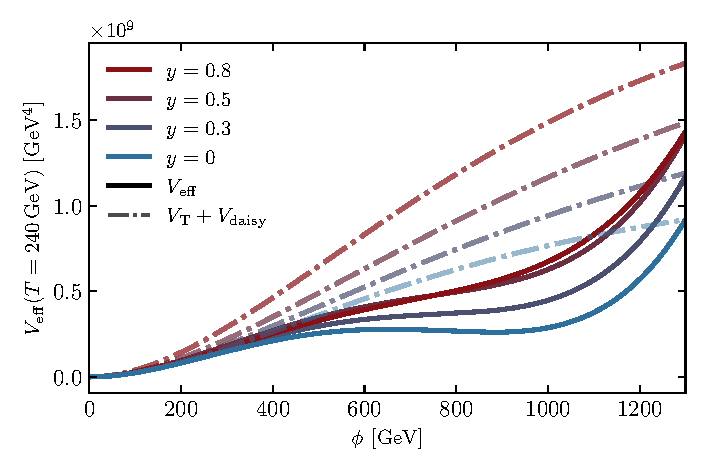
\includegraphics[width=\textwidth]{thesisplots/lisa/thesis_LISA_1.pdf}
	\caption{Total effective potential (solid) and finite temperature part (dot-dashed)
		for $g=0.67, \lambda=0.0035, v_{\phi} = 1\,\text{TeV}$ and $T = 240\,\text{GeV}$, for varying
		values of $y$.}
	\label{fig:potential}
\end{figure}

In addition to encoding the properties of the phase structure, the effective potential also provides information about the stability of the true vacuum after the \ac{PT} occurs. In fact, a new feature becoming important for non-zero Yukawa couplings is that for low values of $\lambda$ and $g$ the potential can become unbounded from below~\cite{Weinberg:1976pe}. To ensure vacuum stability we require that no deeper vacua are present at zero temperature. \graffito{Fermions destabilize the vacuum} The requirement of a \ac{DSPT} already implies that $V_\text{eff}(0) > V_\text{eff}(v_\phi)$. Hence, it is sufficient to check whether there exist vacua with lower potential energy for large field values, i.e.~whether $V_\mathrm{eff}(\phi) < V_\mathrm{eff}(v_\phi)$ for $\phi \gg v_\phi$. In our analysis, we explicitly exclude such parameter points.

It is well known that the one-loop, daisy-resummed calculation of the effective potential can suffer from large theoretical uncertainties, foremost sourced by a large renormalization scale-dependence~\cite{Croon:2020cgk}. A possibility to improve upon those uncertainties is to systematically resum higher orders of the thermal masses in the effective field theory framework of dimensional reduction~\cite{Ginsparg:1980ef}. In order to validate our simpler approach, we therefore also implemented our model in \texttt{DRalgo}~\cite{Ekstedt:2022bff}, which automates the task of \graffito{\texttt{DRalgo} validated $V_\mathrm{eff}(\phi)$} dimensional reduction. We calculate the critical temperature in both our four-dimensional implementation and the reduced three-dimensional theory for the parameter space where we expect a \ac{FOPT}. In the regime where the effective field theory is valid ($T \gg m_{\phi}$) we find that the two results agree very well. We therefore conclude that we can use the computationally more economical approach of using the 1-loop, daisy-resummed effective potential stated in eq.~\eqref{eq:Veff} within the following calculations.

\subsection{Properties of the phase transition}
\label{sec:PT}



\begin{figure}[t]
	\centering
	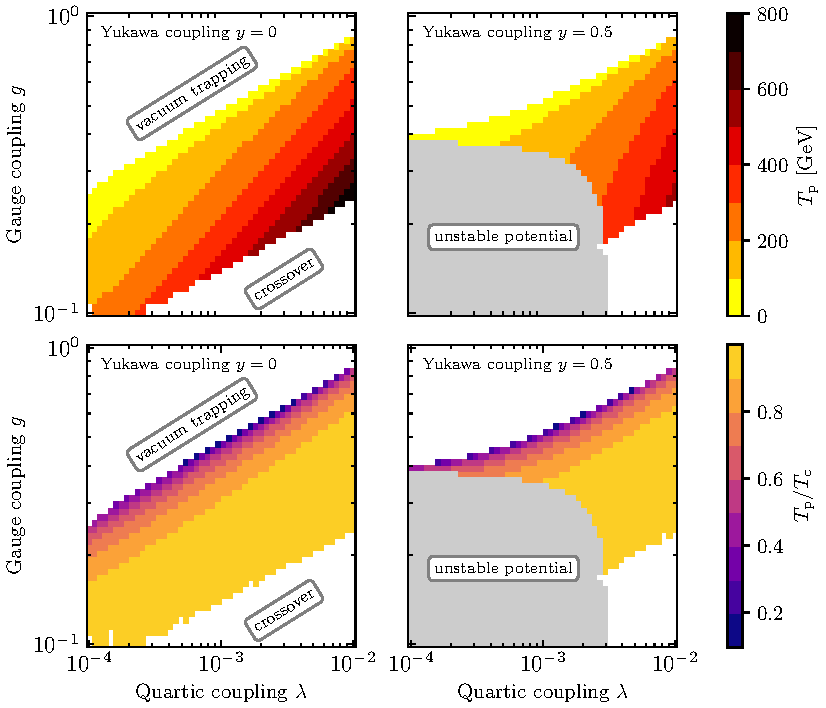
\includegraphics[width=\textwidth]{thesisplots/lisa/thesis_LISA_2}
	\caption{The percolation temperature $T_\perc$ (top) and the ratio of percolation temperature and critical temperature $T_\perc/T_\crit$ (bottom) in the $\lambda-g$ plane for Yukawa couplings of $y=0.0$ (left) and $y=0.5$ (right) and a vev of $v_\phi = 1\, \text{TeV}$. The colored band shows the parameter region where a first-order PT is possible.}
	\label{fig:GWparams-T}
\end{figure}

Next, we want to study the dependence of the percolation temperature $T_\text{p}$ (see eq.~\eqref{eq:falsvacfrac}) and the critical temperature $T_\crit$ on the model parameters. We define the critical temperature as the temperature at which the minimum of the effective potential with non-vanishing \ac{vev} becomes a global minimum.

The dependence of the percolation temperature $T_\perc$ on the model parameters is shown in fig.~\ref{fig:GWparams-T}. In the top panels $T_\perc$ is displayed as a function of the quartic coupling $\lambda$ and gauge coupling $g$ for two values of the Yukawa coupling, $y = 0$ (left) and $y = 0.5$ (right). There is a strong correlation between the values of $\lambda$ and $g$ that produce a \ac{FOPT}, with lower values of $T_\perc$ in the top-left end of the allowed band, and higher values of $T_\perc$ in the bottom-right. The disallowed areas correspond to parameter regions where the transition is not first-order or does not occur at all. These effects are better illustrated in the bottom panels, where the color scale indicates the ratio $T_\perc/T_\crit$ in the same parameter plane. The amount of supercooling of the transition is largest when $T_\perc$ is much lower than $T_ \crit$ and smallest when both temperatures almost coincide. For the points above the colored contours, \graffito{Supercooling for high $g$ and low $\lambda$} the potential barrier becomes so large that the bubble nucleation rate is too low for the transition to reach percolation; the region below instead indicates a smooth crossover transition in which no bubbles form since the potential does not develop a barrier between the phases. For non-zero values of the Yukawa coupling $y$, the enhanced thermal corrections in the effective potential cause a delay of the development of the true vacuum (cf.~fig.~\ref{fig:potential}), thereby decreasing the value of $T_\perc$. The vacuum also becomes deeper due to the Yukawa coupling, which increases the tunneling rate close to the supercooled region, and thus slightly larger values of $g$ are within the allowed band. The gray shaded regions, finally, indicate parameter combinations where the potential is unstable.

\begin{figure}[t]
	\centering
	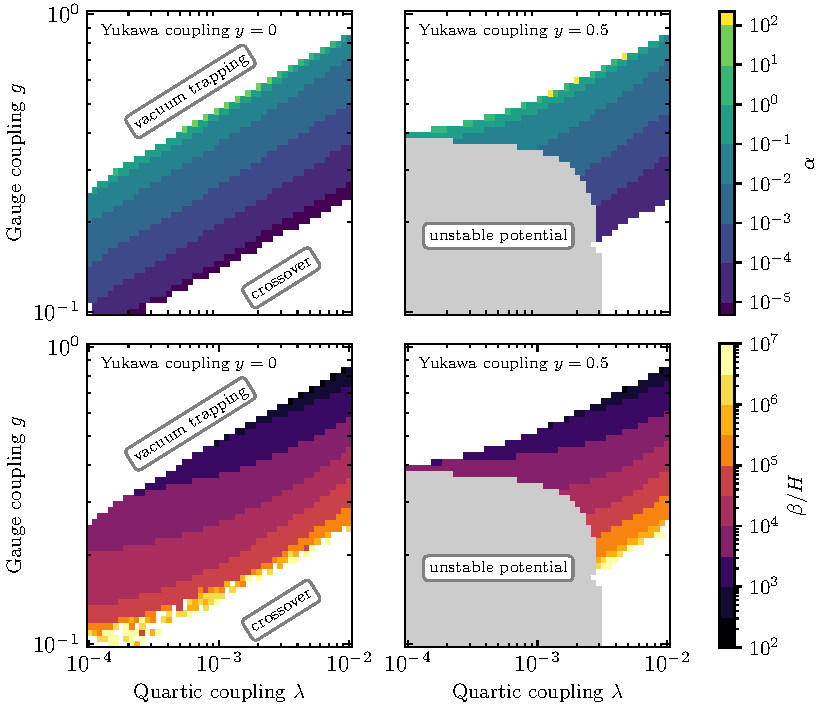
\includegraphics[width=\textwidth]{thesisplots/lisa/thesis_LISA_3}
	\caption{The transition strength $\alpha$ (top) and speed $\beta/H$ (bottom) of the \ac{PT}, in the $\lambda-g$ plane for $y = 0$ (left) and $y = 0.5$ (right), with $v= 1\,\text{TeV}$ and $\xi = 1$.}
	\label{fig:GWparams-alpha-beta}
\end{figure}

In fig.~\ref{fig:GWparams-alpha-beta} we show how the transition strength $\alpha$ (see eq.~\eqref{eq:alpha}) and transition speed $\beta/H$ (see eq.~\eqref{eq:betaH}) depend on the model parameters, $\lambda$, $g$ and $y$. The \ac{PT} is relatively \graffito{Strong and slow transitions are possible} strong for most of the allowed region $\alpha \in (10^{-2}, 10^2)$ and it is particularly strong close to the supercooled limit, where percolation is delayed ($T_\perc \ll T_\crit$). On the other hand, the speed of the \ac{PT} $\beta/H$ becomes smaller in the supercooling limit, reaching values of $\beta/H \approx 10^2 - 10^3$. Both are indicators for a strong \ac{GW} background.


\subsection{The gravitational wave spectrum}
\label{sec:GWspec}

The spectrum of \acp{GW} in our scenario is produced dominantly through bulk fluid motion in the reheated plasma due to the large velocity-dependent friction from the emission of soft dark photons in the bubble wall, yielding a terminal bubble wall velocity~\cite{Bodeker:2017cim,Gouttenoire:2021kjv, Azatov:2023xem}. A discussion of this argument can be found in appendix~\ref{app:darkwalls}. As the case of runaway bubbles can hence be excluded, we neglect the contribution of bubble collisions to the \ac{GW} signal. Since the onset of turbulence as a GW source is not yet understood well enough to make quantitative statements~\cite{Caprini:2019egz}, and often requires complicated lattice simulations~\cite{RoperPol:2019wvy}, we conservatively consider sound waves the only relevant source of \acp{GW} emitted during the \ac{PT}. Therefore, the \ac{GW} spectrum is exclusively determined by the previously discussed set of parameters $\bc{\alpha, \beta/H, T_\perc}$. We use the semi-analytical approximation provided in eq.~\eqref{eq:sw} to compute the peak frequency and \ac{GW} spectrum from sound shell collisions.

A strong \ac{GW} signal typically requires sizable $\alpha$ and values of $\beta/H$ that are not too large. From the discussion of fig.~\ref{fig:GWparams-alpha-beta}, a strong \ac{FOPT} implies large but perturbative values of both $g$ and $\lambda$. Too small values of these two couplings would imply very large values of $\beta/H$ and correspondingly weak \ac{GW} signals, and even cause issues of vacuum stability (for large $y$, cf.~right panel of fig.~\ref{fig:GWparams-alpha-beta}). This in turn induces an upper limit on the value of $y$ as large values would cause an \graffito{Obtaining strong \acp{GW} requires strong couplings} unstable vacuum for any perturbative value of $g$ and $\lambda$. As will be seen below in section \ref{sec:relic}, successfully producing the right \ac{DM} relic density requires $m_\chi \gtrsim m_\phi$, which implies a lower limit $y > 2\sqrt{\lambda}$. Lastly, the \ac{vev} $v_\phi$ is chosen in a range that produces \acp{GW} in the frequency range of near-future \ac{GW} observatories, such as \ac{LISA}.

Consequently, we randomly draw parameters from distributions that are logarithmically flat within the following ranges: $0.1 \leq g \leq 1$, $10^{-4} \leq \lambda \leq 10^{-2}$, $0.01 \leq y \leq 0.7$ and $10^{-3} \, \text{GeV} \leq v_{\phi} \leq 10^{3}\, \text{GeV}$. We then discard parameters that cause  the vacuum to be unstable, that do not predict a \ac{FOPT}, or for which the \ac{PT} is too supercooled and never percolates, thereby removing $82\%$ of the points drawn. \graffito{Strong supercooling for 1\% of points} The remaining 18\% of parameter points all feature a \ac{FOPT} with a corresponding \ac{GW} signal. However, since the percolation temperature is very sensitive to small changes in the couplings, the \ac{PT} is only strong enough to give an observable \ac{GW} signal in certain small regions of parameter space. Indeed, only about 1\% of parameter points from the original sample feature strong supercooling ($T_\perc / T_\text{c} < 0.5$).

We can quantify the fine-tuning required to obtain an observable \ac{GW} signal by interpreting our parameter scan as a sample drawn from the prior distributions of the parameters. We then find that out of the parameter points that give a \ac{FOPT}, only about 0.8\% would be observable with \ac{LISA}, whereas this number increases to 10\% if we select parameter points that give a strongly supercooled \ac{PT}. For the parameter ranges \graffito{Out of these, 10\% can be seen with \ac{LISA}} that we consider (in particular of $v_\phi$) none would be observable with \acp{PTA} or the Einstein Telescope. We note that these numbers do not correspond to rigorously calculated posterior probabilities, but rather rough estimates based on sampling densities. More precise estimates would require a different sampling strategy (see e.g.~\cite{AbdusSalam:2020rdj}), which is beyond the scope of this chapter.

We emphasize that these numbers are largely independent of the choice of priors as long as we select only parameter points that predict any kind of \ac{FOPT}. The probability to find parameter points that give a \ac{FOPT} does however depend sensitively on the choice of priors. If we were to extend the prior ranges for all parameters to lower couplings, the volume of parameter space without a \ac{FOPT} would grow significantly. Choosing for example $g > 0.01$ (instead of 0.1), $\lambda > 10^{-5}$ (instead of $10^{-4}$) and $y > 10^{-3}$ (instead of 0.01) would decrease the fraction of parameter points with a \ac{FOPT} from 18\% to 6\%. Out of these, 0.7\% would be observable by \ac{LISA}, which increases to 8.5\% when considering \graffito{Dependence on prior choices} only points with a strongly supercooled \ac{PT}. As expected, our results are not very sensitive to different prior choices as we find that points that already have a \ac{FOPT} have a roughly equivalent probability of being visible at \ac{LISA} regardless of the parameter ranges. In later sections, we will discuss how
these numbers change when imposing additional constraints on the \ac{DS}, such as the relic density requirement.

Finally, when studying the effects of thermalization in our model in section \ref{sec:thermalization} it will be convenient to identify a benchmark scenario with the right properties for the \ac{PT} and \ac{DM} relic abundance. For reference the benchmark point is given in table \ref{tab:BP}.

\begin{table}[h]
	\centering
	\begin{tabular}{C{0.07\textwidth}C{0.12\textwidth}C{0.07\textwidth}C{0.12\textwidth}C{0.12\textwidth}C{0.1\textwidth}C{0.12\textwidth}}
		\toprule
		 $g$ & $\lambda$ & $y$ & $v_\phi$ & $m_{\chi}$ & $m_\phi$ & $m_{A'}$\\
		\midrule
		 $0.67$ & $0.0035$ & $0.62$ & $430\,\text{GeV}$ & $189\,\text{GeV}$ & $36\,\text{GeV}$ & $288\, \text{GeV}$ \\
		\bottomrule
	\end{tabular}
	\caption{Benchmark point used for discussing the thermalization of visible and dark sector.}
	\label{tab:BP}
\end{table}



\section{The dark sector relic density}
\label{sec:relic}

\begin{figure}[t!]
	\centering
	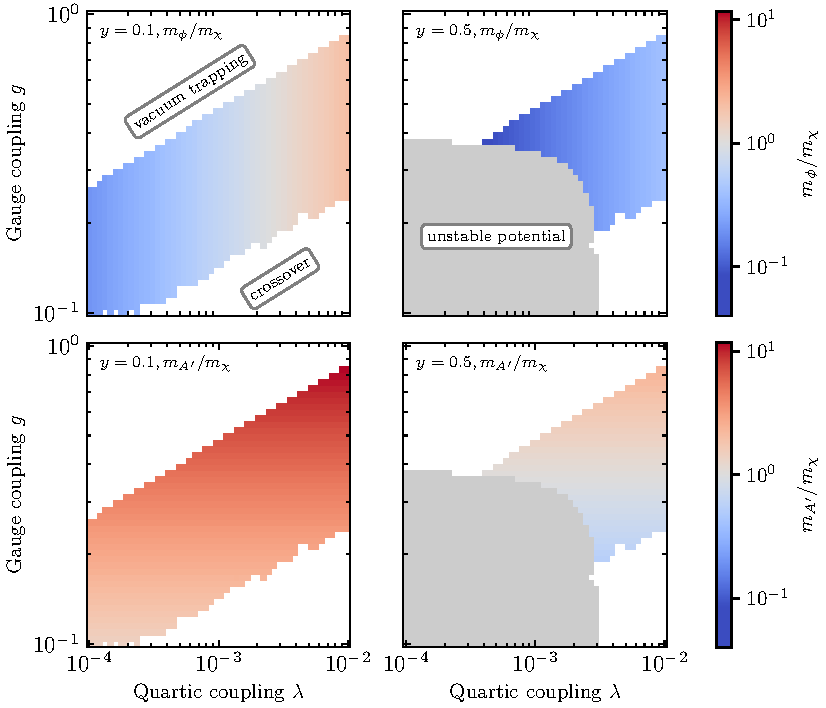
\includegraphics[width=\textwidth]{thesisplots/lisa/thesis_LISA_4}
	\caption{
		The upper (lower) panels show the ratio of the dark Higgs boson mass $m_\phi$ (the dark photon mass $m_{A'}$) to the mass of the DM fermion $m_\chi$ for $y = 0.1$ (left) and $y = 0.5$ (right), as a functions of the gauge coupling $g$ and the self-interaction $\lambda$. Note that these ratios are independent of the dark Higgs \ac{vev}.}
	\label{fig:mass_ratios}
\end{figure}

During the \ac{PT}, the \ac{DS} particles $\chi$, $\phi$ and $A'$ all obtain masses proportional to the dark Higgs \ac{vev} $v_{\phi}$. In the parameter regions of interest for a strong \ac{FOPT}, we generally find $g > \sqrt{2\lambda}$ and $g > y/\sqrt{2}$ and hence the dark photon is usually the heaviest state in the \ac{DS}, cf.~eq.~\eqref{eq:masses}. Depending on the value of the Yukawa coupling $y$, the lightest \ac{DS} particle will instead be either the \ac{DM} fermion or the dark Higgs boson, as shown in fig.~\ref{fig:mass_ratios}. The \ac{DS} equilibrates soon after the \ac{PT} (see section~\ref{sec:equilibrium} for a more detailed discussion). Typically, the heaviest particles will then first drop out of equilibrium as their \graffito{$m_\chi < m_\phi < m_{A^\prime}$ or $m_\phi < m_\chi < m_{A^\prime}$} number densities become strongly suppressed. The relic abundance of the dark fermions $\chi$ is thus determined through a freeze-out process~\cite{Lee:1977ua} in the usual way. We assume that the dark photon is unstable, decaying for example through kinetic mixing, and therefore does not contribute to the \ac{DM} relic density (unlike the case studied in ref.~\cite{Kanemura:2023jiw}).

In our model there are three possible \ac{DM} annihilation processes that are relevant for setting the \ac{DM} abundance: $\chi \chi \to \phi \phi$, $\chi \chi \to \phi A'$ and $\chi \chi \to A' A'$. If the \ac{DM} fermion is the lightest particle in the \ac{DS}, annihilation
into other \ac{DS} states is kinematically forbidden for vanishing kinetic energy, such that the annihilation cross section becomes exponentially suppressed at low temperatures. In this so-called `forbidden' regime~\cite{DAgnolo:2015ujb}, a relic abundance in accordance with observations requires that all mass scales must \graffito{Available \ac{DM} annihilation channels} be correspondingly smaller, or the relevant couplings (much) larger. For the parameter values we are interested in here, it is therefore typically necessary for the \ac{DM} particle to be heavier than the dark Higgs boson, which in turn requires a sizable Yukawa coupling $y$. For even heavier \ac{DM}, with $2 m_\chi \gtrsim m_\phi + m_{A'}$, the annihilation channel $\chi \chi \to \phi A'$ opens up. This process is a highly relevant contribution, once kinematically accessible, as it proceeds via an $s$-wave; the annihilation into a pair of dark Higgs bosons, $\chi\chi\to\phi\phi$, on the other hand,
only proceeds via a $p$-wave. 

To compute the \ac{DM} relic density, we have calculated the amplitudes for all three processes, see appendix~\ref{app:annihilation}, and implemented them in \ds~\cite{Bringmann:2018lay}, which \graffito{We solve Boltzmann equations with \ds} calculates the thermal averages and solves the full Boltzmann equation~\cite{Gondolo:1990dk}. While \ds\ allows precision calculations of the relic density in a fully secluded \ac{DS} with a varying  temperature ratio $\xi$ between the dark and the \ac{SM} sector, cf.~ref.~\cite{Bringmann:2020mgx}, we will set  $\xi = 1$ for the purpose of this section. We will revisit this assumption of thermal equilibrium between the two sectors in section~\ref{sec:equilibrium}.

\begin{figure}[t!]
	\centering
	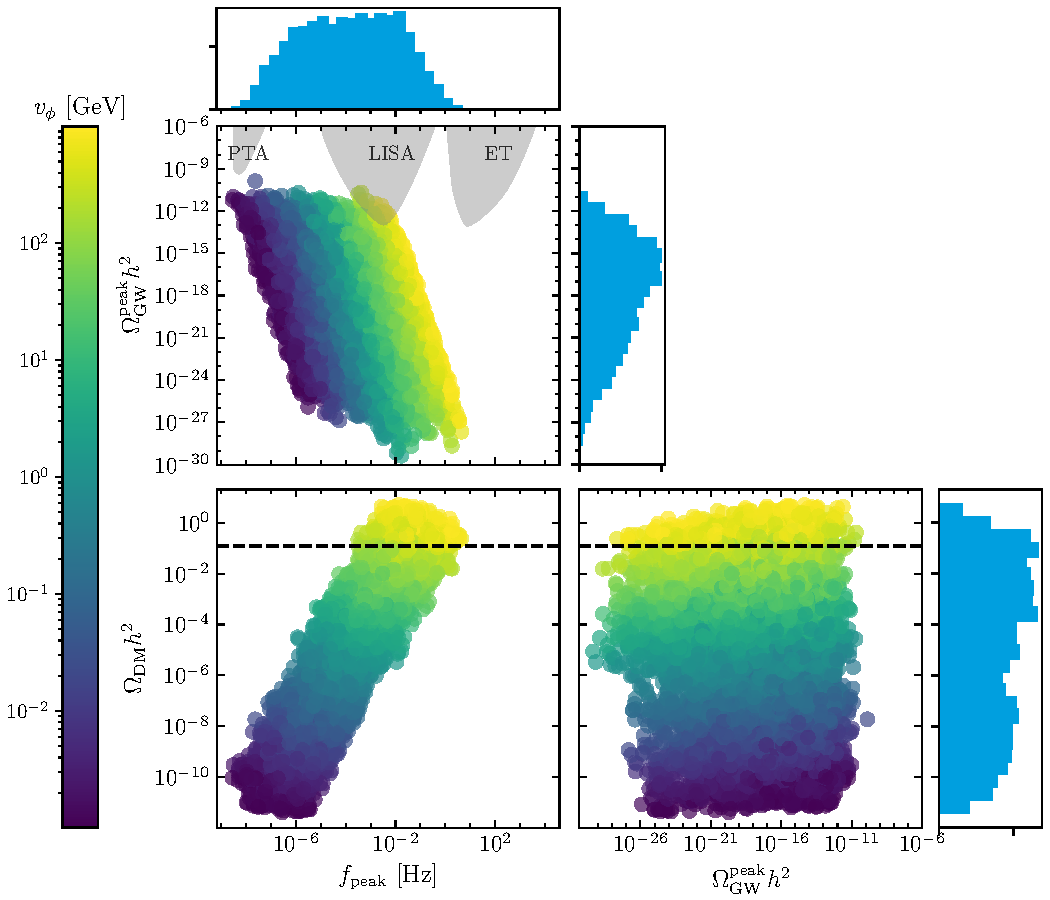
\includegraphics[width=\textwidth]{thesisplots/lisa/thesis_LISA_5}
	\caption{Scatter plots and 1D distributions of the \ac{DM} density $\Omega_\mathrm{DM} h^2$, the \ac{GW} peak amplitude $\Omega_\mathrm{GW} h^2$, and the peak frequency $f_\mathrm{peak}$. For comparison, the dashed line shows the observed \ac{DM} density, $\Omega_\DM h^2 = 0.12$~\cite{Planck:2018vyg}; gray shaded areas show the \ac{PLI} sensitivities~\cite{Breitbach:2018ddu} of \acp{PTA}, \ac{LISA} and \ac{ET}, respectively.}
	\label{fig:triangle-unrestr}
\end{figure}

We show the results from the parameter scan described in section~\ref{sec:GWspec} in fig.~\ref{fig:triangle-unrestr}. The three two-dimensional scatter plots show the correlation between the \ac{DM} relic density $\Omega_\DM h^2$, the peak frequency $f_\peak$ as well as the peak amplitude $\Omega_\GW^\peak h^2$. One can immediately see that $\Omega_\DM$ and $\Omega_\GW^\peak$ are not tightly correlated (with a correlation coefficient of 0.20), while there exists a clear connection between the \ac{DM} relic density and the peak frequency (with a correlation coefficient of 0.85). We \graffito{Tight correlation between $\Omega_\mathrm{DM}$ and $f_\mathrm{peak}$} can trace this correlation back to the fact that both quantities are determined by the dark Higgs \ac{vev} $v_{\phi}$ (indicated by the color of each point). A smaller value of $v_{\phi}$ implies a smaller \ac{DM} mass and therefore a larger annihilation cross section, which in turn results in a smaller relic density. At the same time, a smaller $v_{\phi}$ also implies a smaller percolation temperature, and hence a smaller peak frequency. The strength of the \ac{PT}, on the other hand, depends on the details of the effective potential, and can vary over many orders of magnitude for any given value of $v_{\phi}$.

We complement these scatter plots by showing distributions of the derived quantities, in the form of histograms based on our random scan described above. For example, one can infer that most samples \graffito{Typically $\Omega_\mathrm{GW}^\mathrm{peak} h^2 \approx 10^{-16}$} drawn in our setup correspond to a peak \ac{GW} signal strength of $\Omega_\GW^\peak h^2 \approx 10^{-16}$, i.e.~a few orders of magnitude below the \ac{PLI} sensitivity of near-future \ac{GW} observatories (indicated as gray shaded areas). Note also that the \ac{DM} density caps at $\Omega_\DM h^2\approx10$, which would already correspond to an overclosed universe; even higher values are avoided by our prior choice, in particular the upper bound on $v_\phi$ and the lower bound on $y$.

\begin{figure}[t!]
	\centering
	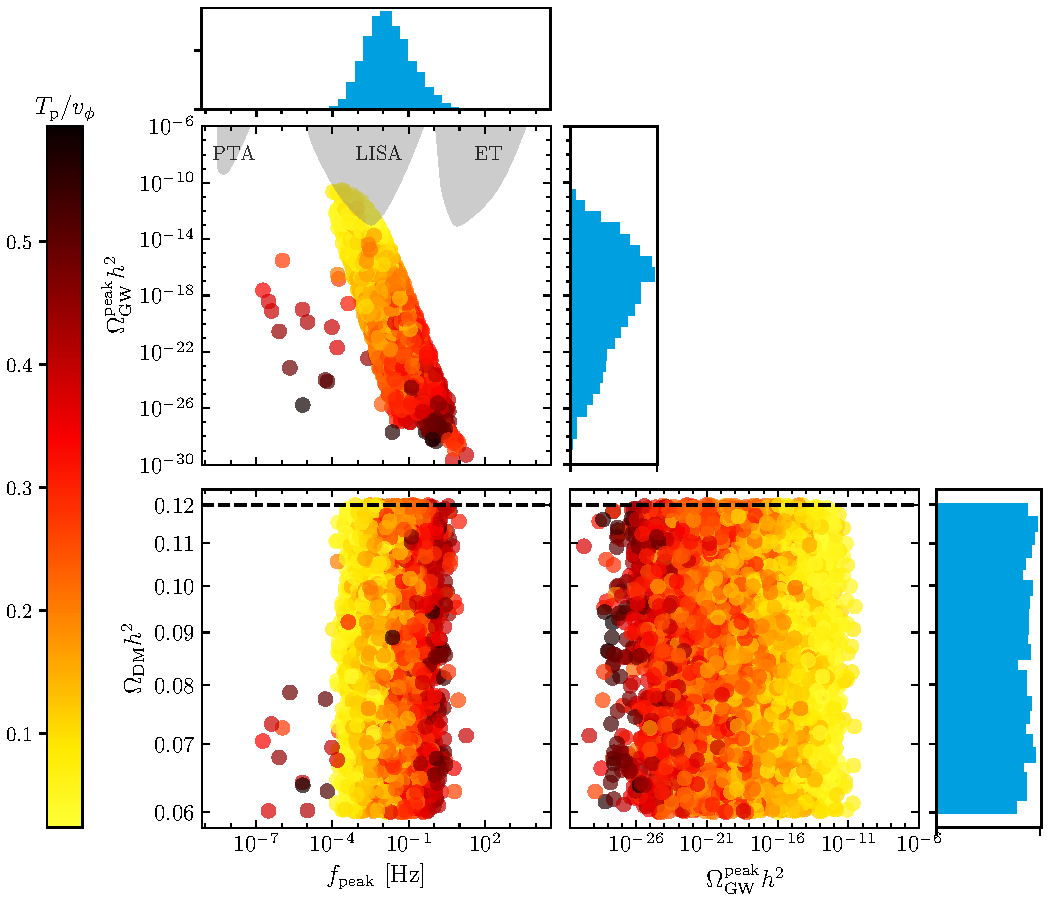
\includegraphics[width=\textwidth]{thesisplots/lisa/thesis_LISA_6}
	\caption{Scatter plots and 1D distributions as in fig.~\ref{fig:triangle-unrestr}, but with the additional constraint $0.06 \, \leq \Omega_\DM h^2 \leq 0.12$. Here, the color scale does not encode the \ac{vev}, but the ratio of percolation temperature $T_\perc$ to the \ac{vev} $v_\phi$, thus indicating the amount of supercooling.}
	\label{fig:triangle-restr}
\end{figure}

In fig.~\ref{fig:triangle-restr} we show the result of sharpening the relic density requirement by requiring that $0.06 \, \leq \Omega_\DM h^2 \leq 0.12$. Demanding in this way that the fermionic \ac{DM} candidate in our model constitutes the dominant form of \ac{DM}, the predicted range of peak frequencies of the \ac{GW} signal shrinks significantly---as expected from the discussion above. Interestingly, almost all viable parameter points now predict a peak frequency between $0.1 \, \mathrm{mHz}$ and $100 \, \mathrm{mHz}$, largely overlapping with the frequency range to which \ac{LISA} is sensitive. In fact, the peak frequencies for those parameter points that result in the strongest signal are \graffito{Require $\Omega_\mathrm{DM}h^2 \simeq 0.12$: \acp{GW} in \ac{LISA} band!} the same as those where \ac{LISA} is most sensitive. This striking correlation is a non-trivial feature of our model and constitutes one of our main results. Let us note that a few points remain that predict peak frequencies outside the \ac{LISA} band. Much smaller values of $f_\mathrm{peak}$, in particular, correspond to parameter points in the `forbidden' regime, $m_\chi < m_\phi$, where \ac{DM} annihilations are exponentially suppressed at small temperatures. Smaller values of $v_\phi$ (and hence smaller temperatures of the \ac{PT}) can then still result in the correct \ac{DM}
relic abundance, but only at the cost of a significant tuning between the various couplings (as reflected by the rareness of such parameter points, cf.~the $f_\mathrm{peak}$ histogram at the top of the plot).

In contrast to fig.~\ref{fig:triangle-unrestr}, where the color coding of each point represents the dark Higgs \ac{vev}, the points in fig.~\ref{fig:triangle-restr} are colored according to the percolation temperature of the \ac{PT}, normalized to the \ac{vev} $v_\phi$. Doing so allows us to confirm that the peak amplitude \graffito{Observability requires strong supercooling} of the \ac{GW} spectrum is determined primarily by the amount of supercooling. In other words, if the \ac{PT} is delayed by a large potential barrier, the strength of the \ac{PT} increases, yielding strong \ac{GW} amplitudes (as expected from figs.~\ref{fig:GWparams-T} and~\ref{fig:GWparams-alpha-beta}). As discussed in section~\ref{sec:GWspec}, the predictions for the \ac{PT} properties vary a lot with small changes of the model parameters, and thus only certain regions of the parameter space predict a strong \ac{FOPT}. For this reason, our model cannot in general guarantee a strong \ac{PT}, and thus a \ac{GW} signal that is visible with next-generation \ac{GW} observatories.

We can make this statement more precise if we interpret the sampling distributions of the model parameters as prior probabilities (as we did in section~\ref{sec:GWspec}), such that the density of points in figs.~\ref{fig:triangle-unrestr} and~\ref{fig:triangle-restr} can be interpreted as probability distributions for the observables under consideration. As before, this makes it possible to quantify the
amount of fine-tuning required to obtain a strong \ac{FOPT}, through the fraction of points with a \ac{FOPT} that predict a
signal observable with \ac{LISA}. If we do not impose the relic \graffito{3\% of points with $\Omega_\mathrm{DM}h^2 \simeq 0.12$ can be seen with \ac{LISA}} density requirement (fig.~\ref{fig:triangle-unrestr}), only 0.8\% of points
with a \ac{FOPT} predict a \ac{GW} signal visible at \ac{LISA}, whereas this fraction increases to 3\% once the relic density requirement is included (fig.~\ref{fig:triangle-restr}). If we restrict ourselves to parameter points with a strongly supercooled \ac{PT}, the fraction of observable parameter points increases from 10\% to 35\%. Again, we have checked that this number is not very sensitive to our choice of parameter ranges.



\section{Thermalization of the two sectors}
\label{sec:equilibrium}

In this section we revisit the assumption that the temperature ratio of the dark and visible sectors is $\xi = 1$ throughout the \ac{PT}. To do so, we first need to understand the evolution of the \ac{DS} temperature during the \ac{PT}, and convince ourselves that the
\ac{DS} quickly thermalizes with itself afterwards, such that the \ac{DS} states remain in kinetic equilibrium with each other until after \ac{DS} freeze-out (i.e.~chemical decoupling). However, \graffito{Let's drop the $\xi = 1$ assumption} it is not necessarily the case that also the \ac{SM} states are in kinetic equilibrium with the \ac{DS}, such that their temperature may differ from the one of the \ac{DS} both before and after the \ac{PT}. We therefore discuss the various processes that allow for the exchange of energy and entropy between the dark and the \ac{SM} sector, and the resulting Boltzmann equations. This enables us to identify the necessary portal couplings for efficient thermalization. For
the case of delayed thermalization, after the end of the \ac{PT}, we calculate the resulting dilution of the \ac{GW} signal due to the injection of entropy into the \ac{SM} thermal bath.

For the purpose of illustration, we will in this section consider a specific benchmark point that we selected from the random parameter scan discussed previously (see table~\ref{tab:BP}). For $\xi=1$, the parameters of this point lead to $\alpha = 0.258$, $\beta/H=874$,
$T_\nuc=39.7\,\text{GeV}$, $T_\perc=39.1\,\text{GeV}$, $f_\peak=3\,\text{mHz}$, $\Omega_\DM h^{2} = 0.117$, and $\Omega_\GW^\peak h^2=3\cdot10^{-13}$. The rationale behind \graffito{A benchmark point} choosing this benchmark point is that (\textit{i}) the observed \ac{DM} relic abundance is reproduced (for $\xi = 1$), and that (\textit{ii}) the \ac{PT} is sufficiently strong in order to obtain an observable signal in \ac{LISA}. We have explicitly checked that our choice is representative in the sense that other points fulfilling these two criteria lead to a very similar temperature evolution and resulting predictions.

\subsection{The dark sector temperature}

As the bubbles of the broken phase expand, more and more \ac{DS} particles will pass through the bubble walls and enter the new phase. In the process, not only their rest masses but also their kinetic energies increase dramatically, by converting the vacuum energy of the dark Higgs field stored in the false vacuum. Here we neglect the small fraction of the energy density that is converted into \acp{GW} and assume that the bubble walls have already \graffito{We can ignore bubble filtering} reached their terminal velocity, such that no energy is needed for their acceleration. As we have learned in the previous section, in particular, the energy density of  \acp{GW} produced in the \ac{PT} is bounded by $\Omega_\GW^\peak h^2 < 10^{-10}$ and can therefore safely be ignored. We also neglect the effect of bubble filtering~\cite{Baker:2019ndr, Chway:2019kft}, i.e.~we assume that all \ac{DS} particles can enter the new phase. This is a good approximation for sufficiently fast bubble walls, see appendix~\ref{app:darkwalls} for details.

Since the different particle species in the \ac{DS} were all relativistic before the \ac{PT}, their number densities immediately after
the \ac{PT} will  be comparable, even though their masses will now be very different. Indeed, for strongly supercooled \acp{PT} the dark photons (and possibly also the \ac{DM} particles) will typically \graffito{Particles behind the wall are out of equilibrium} have a large mass  compared to the temperature of the plasma, such that their equilibrium number density would be Boltzmann-suppressed. In other words, right after the \ac{PT} the \ac{DS} finds itself far away from thermal equilibrium. Nevertheless, interactions between the different \ac{DS} particles are rather strong, and hence the heavier particles are expected to annihilate rapidly into lighter ones, thereby restoring equilibrium.

As we will show below, the time required to \graffito{Energy conservation fixes the broken-phase temperature} reach equilibrium is negligible compared to the duration of the \ac{PT}, such that we can to a very good approximation define a \ac{DS} temperature of the broken phase $\TDSbro$ immediately after the \ac{PT}. This temperature is obtained from the temperature of the symmetric \ac{DS} phase $\TDSsym$ using energy conservation:
\begin{align}
	\rho_\text{vac}(\TDSbro) + \rho_\DS(\TDSbro) =  \rho_\text{vac}(\TDSsym) + \rho_\DS(\TDSsym) \, . \label{eq:energy_cons}
\end{align}
Here, $\TDSbro$ denotes the temperature in the broken phase and
\begin{align}
	\rho_\DS(\TDSbro) = \frac{\pi^2}{30} \, g_{\DS}(\TDSbro) \, \TDSbro^4 \,  ,
\end{align}
where $g_{\DS}(T)$ takes into account the $T$-dependence stemming both from thermal (field-dependent) masses and the minimum of the effective potential. Eq.~\eqref{eq:energy_cons} can easily be solved numerically for $\TDSbro$ for a given $\TDSsym$.

In practice, we find that slightly different temperatures $\TDSbro$ of the broken phase are obtained when solving the equation taking $\TDSsym= T_\perc$ or $\TDSsym = T_\nuc$. This is because the energy density of the broken phase redshifts differently from the symmetric phase. We have therefore implemented a more detailed \graffito{We set $T_\mathrm{d,sym}$ to percolation temperature} calculation, which tracks the temperature of the symmetric and broken phases from bubble nucleation to percolation and applies eq.~\eqref{eq:energy_cons} at each time step to the fraction of the universe entering the broken phase. Here the energy in the bubble walls, which for relativistic bubble wall velocities redshifts like radiation~\cite{Gouttenoire:2023naa}, is included in the energy of the symmetric phase. We find that this more careful treatment gives very similar results to simply applying eq.~\eqref{eq:energy_cons} at $\TDSsym = T_\perc$. We therefore use the latter prescription in the following when computing the temperature of the \ac{DS} after the \ac{PT}.

For our benchmark point, we find that the energy density of the \ac{DS} before the \ac{PT} is dominated by vacuum energy (see fig.~\ref{fig:hubble-parameter}). In the broken phase, on the other hand, the vacuum energy is very small and quickly relaxes to a value very close to its zero temperature value as the temperature decreases further. This difference in vacuum energy leads to a substantial reheating of the \ac{DS}, which, as a result, is \graffito{Reheating of the \ac{DS} leaves $\phi$ relativistic} hotter than the \ac{SM} sector after the \ac{PT}. For our benchmark point, we find that if the two sectors have equal temperature before the \ac{PT}, in the broken phase the \ac{DS} temperature will be larger by a factor of about 1.3. This reheating of the \ac{DS} typically ensures that the dark Higgs bosons will be relativistic immediately after the \ac{PT}.

\begin{figure}[t]
	\centering
	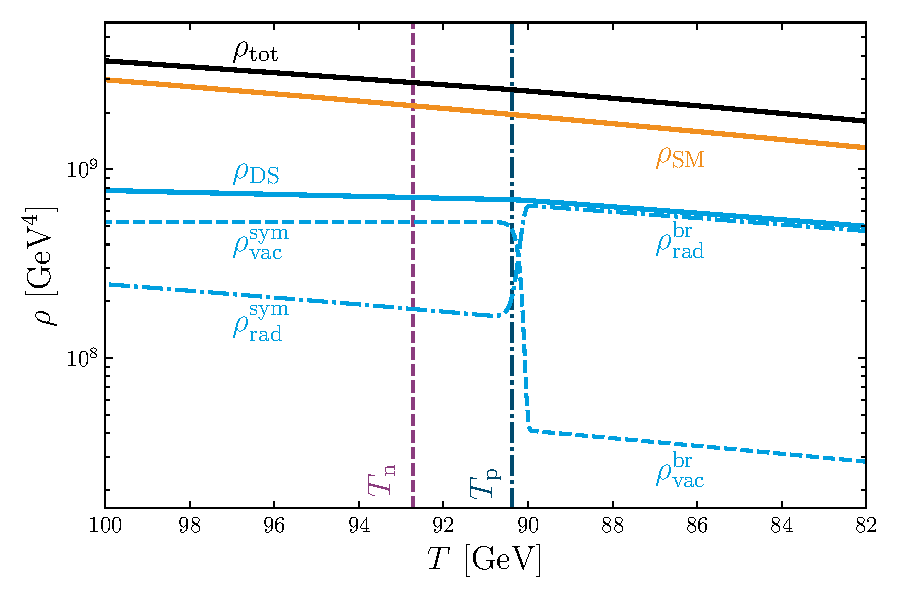
\includegraphics[width=0.9\textwidth]{thesisplots/lisa/thesis_LISA_7}
	\caption{Contributions to the energy density around the \ac{PT} for our benchmark point, as a function of the \ac{SM} temperature and for a temperature ratio $\xi = 1$. The energy densities in the symmetric and broken phase of the \ac{DS} have two contributions, namely the energy of the particles (`rad') and the potential energy of the scalar field (`vac').}
	\label{fig:hubble-parameter}
\end{figure}


\subsection{Thermalization within the dark sector}
\label{sec:thermalization}

In the discussion above we have assumed that the \ac{DS} can be characterized by a common temperature shortly after the \ac{PT}. To justify this approach, we need an estimate of the time $\tau$ required to reach this equilibrium state and show that it is sufficiently
small. For this purpose, we calculate the interaction rate for each \ac{DS} state $X$ in thermal equilibrium:
\begin{align}
	\Gamma_X = \sum_Y \langle \sigma_{XY} v \rangle n_Y^\mathrm{eq} \,,
\end{align}
where the sum is over all \ac{DS} states $Y$, $\sigma_{XY}$ denotes the total interaction cross section of $X$ and $Y$, brackets denote thermal averaging (for simplicity calculated by assuming Boltzmann distributions) and $n_Y^\mathrm{eq}$ denotes the equilibrium number density of $Y$. 

A total of 20 different processes contribute to the thermalization of the \ac{DS}, the relative importance of which depends on the specific choice of parameters and the \ac{DS} temperature. In the interest of brevity we refrain from stating the thermalization
rates explicitly. Broadly speaking, we find that $\Gamma_X$ is only a few orders of magnitude smaller than $m_X$. For example, dark Higgs bosons can thermalize via \graffito{20 processes contribute to the \ac{DS} thermalization} self-scattering, i.e.~$\phi \phi \leftrightarrow \phi \phi$, for which the scattering cross section is
$9 \lambda^2 / (8 \pi s)$. For temperatures comparable to the dark Higgs boson mass, we have $s \approx 4 m_\phi^2$ and $n_\phi \approx \zeta(3) m_\phi^3 / \pi^2$, such that $\Gamma_\phi \sim 10^{-7} m_\phi$ for the benchmark point. Interactions of the dark Higgs bosons with dark fermions or dark photons benefit from the larger couplings $y, g \gg \lambda$, but suffer from a Boltzmann suppression if $T_\perc < m_\chi, m_{A'}$.

A rough estimate of the thermalization timescale is then obtained via 
\begin{align}
	\tau = \max_X \, \Gamma_X^{-1} \, .
\end{align}
Given the timescale $\tau$ we can estimate the out-of-equilibrium fraction $F(t)$ of the universe, which describes the relative volume of the universe that entered the broken phase so recently that it has not had enough time to reach thermal equilibrium. The related
false vacuum fraction $P(t)$, cf.~eq.~\eqref{eq:falsvacfrac}, describes the fraction of the universe which has not yet transitioned to the new phase, such that the true vacuum \graffito{The out-of-equilibrium fraction $F(t)$...} fraction is given by $P_\true(t) = 1 - P(t)$. Its time derivative $\dot{P}_\true$ describes the rate with which the volume is transitioning to the true minimum of the potential for a given time $t$. We introduce the quantity
\begin{align}
	F(t) \equiv P(t - \tau) - P(t) > 0\,,
\end{align}
which can hence be interpreted as the volume fraction $\dot{P}_\true \, \Delta t$ that just transitioned to the broken phase within the small thermalization time scale $\Delta t = \tau$, cf.~fig.~\ref{fig:hubble-parameter}. The volume fraction $F$ becomes small exactly when the thermalization timescale $\tau$ is small compared to the transition timescale $1/\beta$, as can be seen from the saddle point approximation of $P(t)$ around the percolation time $t_\perc$:
\begin{align}
	\begin{split}
		F(t) &\approx \exp \left( -0.34 \mathrm{e}^{\beta(t - t_\perc - \tau)} \right) -
		\exp \left( -0.34 \mathrm{e}^{\beta(t-t_\perc)} \right)  \\
		&= \beta \tau \mathrm{e}^{\beta(t - t_\perc)} \exp \left( -0.34 \mathrm{e}^{\beta(t - t_\perc)} \right) \leq 0.37 \beta\tau\, .
	\end{split}
\end{align}
Here, the last term follows by inserting the time at which $F(t)$ peaks, which is found to be $t \approx t_{\perc} - 1.08/\beta$. \graffito{... is always small.} Alternatively, one can interpret $F$ as the volume fraction of a shell around the bubbles with the width of the mean free path of the particles that just entered the bubbles. In the left panel of fig.~\ref{fig:thermalisation} we show $F$ as a function of $T - T_\perc$ for our benchmark point. As expected, we find that $F$ takes its maximal value close to the  percolation temperature $T_\perc$. Nevertheless, even at the peak the value is tiny, implying that the fraction of the universe that is not in thermal equilibrium and therefore cannot be described by a temperature is completely negligible. In the right panel of fig.~\ref{fig:thermalisation} we show the value $F_\perc \equiv F(T_\perc)$ at the percolation temperature for more points from our parameter scan, varying both $g$
and $\lambda$. Similarly we find that for all our cases the thermalization is fast compared to the transition timescale. Even strongly supercooled points, where $F_\perc$ becomes close to unity, are expected to return to equilibrium before freeze-out, since $\beta/H \gg 1$.

\begin{figure}[t]
	\centering
	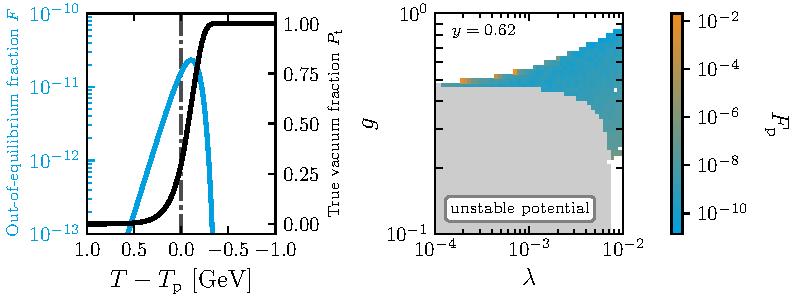
\includegraphics[width=\textwidth]{thesisplots/lisa/thesis_LISA_8}
	\caption{\textit{Left:} The light blue line shows the energy fraction of the \ac{DS} that is out of equilibrium for our benchmark point, as a function of the \ac{SM} photon temperature. For reference, the fraction of the \ac{DS} in the broken phase is given by the
		black line and the percolation temperature as the dashed vertical line. \textit{Right:} Out-of-equilibrium fraction as a function of $\lambda$ and $g$ for $y = 0.62$ and $v_\phi=430\,\text{GeV}$.}
	\label{fig:thermalisation}
\end{figure}

So far, we have throughout assumed that chemical potentials in the \ac{DS} can be neglected after thermalization has taken place. This is certainly a good approximation as long as at least the lightest state in the \ac{DS} has a mass that is small compared to the \ac{DS} temperature, which is typically the case shortly after the \ac{PT}. However, as the universe continues to cool down, this assumption becomes increasingly critical. If we assume that the \ac{DS} cannot transfer its entropy to the \ac{SM} thermal bath, the subsequent evolution depends crucially on whether number-changing \graffito{A note on cannibalistic \acp{DS}} processes of the lightest state, such as $3\phi \to 2\phi$, are efficient enough to maintain chemical equilibrium in the \ac{DS}. If this is the case, the \ac{DS} temperature will decrease much more slowly than the \ac{SM} temperature, and the universe will enter a period of `cannibal' domination~\cite{Pappadopulo:2016pkp,Farina:2016llk}. If, on the other hand, number-changing processes are inefficient, the \ac{DS} will develop large chemical potentials and the universe will eventually enter a period of matter domination. In both cases, the energy and entropy stored in the \ac{DS} must later be transferred to the \ac{SM} heat bath in order to recover radiation domination before neutrinos decouple at $T \approx 2 \, \text{MeV}$, marking the onset of \ac{BBN}~\cite{Bringmann:2023opz}. Neither of these scenarios is very desirable, as the \ac{GW} signals from the \ac{PT} will be strongly diluted in the process~\cite{Ertas:2021xeh}.

We are therefore more interested in the case where the dark and \ac{SM} sector quickly equilibrate after the \ac{PT}, such that their temperatures become equal, chemical potentials become negligible, and the universe evolves approximately as in radiation domination. In the following we discuss the processes that contribute to this process, and we derive the coupling strengths required for it to happen rapidly enough.

\subsection{Thermalization of the dark and visible sector}
\label{sec:DSthermalization}

The conceptually simplest way for the dark and visible sector to exchange entropy and energy is via Higgs
mixing~\cite{Schabinger:2005ei,Patt:2006fw,Weihs:2011wp,Duerr:2016tmh,Li:2023bxy}.\footnote{A second possibility would be to consider kinetic mixing between the dark photon and \ac{SM} hypercharge. However, given that the dark photon is typically the heaviest state in the \ac{DS}, it will be strongly Boltzmann-suppressed at low temperatures, and therefore cannot efficiently keep the two sectors in equilibrium.} Such a mixing arises from an additional term in the scalar potential:
\begin{align}
	V_\text{mix}(H, \Phi) = \lambda_{h\phi} |H|^2 |\Phi|^2 \, .
\end{align}
As long as the \acp{vev} of both Higgs bosons vanish, the dominant \graffito{Thermalization through the Higgs portal} process connecting the two sectors is $H H \to \Phi \Phi$. As soon as one of the two Higgs bosons acquires a \ac{vev}, it can decay into the other one, i.e.~$h \to \Phi \Phi$ (if the electroweak symmetry breaks first) or $\phi \to H H$ (if the dark symmetry breaks first). If kinematically allowed, these decay processes typically dominate over the $2 \to 2$ process for non-relativistic particles.

After both electroweak symmetry and the dark gauge symmetry have been spontaneously broken, the Higgs mixing generates a non-diagonal mass term, which can be rotated away by introducing the mixing angle
\begin{align}\label{eq:mixing-angle}
	\theta = \frac{\lambda_{h\phi} v_\phi  v_h}{m_h^2 - m_\phi^2} \, ,
\end{align}
where we have assumed $\theta \ll 1$ both in order to satisfy experimental constraints on the properties of the \ac{SM}-like Higgs boson and to ensure that thermal corrections from \ac{SM} fields to the effective potential are negligible so that the \ac{DSPT} can be treated separately from the \ac{EWPT}. Both the masses and the \acp{vev}, and hence also the mixing angle, depend on the temperature. As a result of this mixing, the dark Higgs boson obtains couplings to \ac{SM} fermions and gauge bosons proportional to $\theta$. Of the greatest relevance for our discussion will be the decay of dark Higgs bosons into bottom quarks $b$, with a tree-level decay width given by
\begin{align}
	\Gamma_{\phi \to b\bar{b}} = \frac{3  m_\phi m_b^2 \sin^2 \theta}{8\pi v_h^2} \sqrt{1 - \frac{4 m_b^2}{m_\phi^2}} \, .
\end{align}

To calculate the entropy transfer between the dark and visible sector, we define the heat transfer rate
\begin{align}
	\dot{q}_\DS \equiv \dot{\rho}_\phi + 3 H (\rho_\phi + P_\phi) \,,
\end{align}
which is related to the change of entropy density via
\begin{align}
	\dot{s}_\DS = -3  H  s_\DS + \frac{\dot{q}_\DS}{T_\text{d}} \,.
\end{align}
At the same time, the first moment of the Boltzmann equation gives
\begin{align}
	\int \frac{\mathrm{d}^3 p}{(2\pi)^3} E_\phi \, L[f_\phi] = \dot{q}_\DS =  \int \frac{\mathrm{d}^3 p}{(2\pi)^3} E_\phi \, C[f_\phi] \, .
\end{align}
The general expression for the first moment of the collision operator for decays (including relativistic corrections and quantum effects)
was derived in refs.~\cite{Bringmann:2021sth, Bernreuther:2022bdw}. It was shown there that the leading relativistic effects (namely a time dilation of the decay proportional to $1/\gamma$ and an increase of the injected energy by a factor $\gamma$) cancel, and it is therefore a good approximation to assume that the decaying particle is at rest. The integral of the collision operator thus gives
\begin{align}
	\dot{q}_\DS \simeq m_\phi \left(\dot{n}_\phi + 3 H n_\phi\right) \,,
\end{align}
and the evolution of the number density is given by the usual Boltzmann equation
\begin{align}
	\dot{n}_\phi + 3  H  n_\phi = - \Gamma_{\phi \to b \bar{b}}  \, n^\text{eq}_\phi \left(\frac{n_\phi}{n^\text{eq}_\phi} - 1 \right) .
\end{align}
Here $n^\text{eq}_\phi$ denotes the equilibrium number density for $T_\text{d}= T$, whereas the actual number density can be calculated from the \ac{DS} temperature and the assumption of negligible chemical potential. \graffito{Entropy injection to $b$ quarks} Putting everything together, we obtain
\begin{align}
	\dot{s}_\DS = - 3 H  s_\DS - \frac{m_\phi}{T_\mathrm{d}} \, \Gamma_{\phi \to b \bar{b}} \, n^\text{eq}_\phi
	\left( \frac{n_\phi}{n^\text{eq}_\phi} - 1 \right).
\end{align}
A completely analogous equation holds for the evolution of the \ac{SM} entropy density $s_\SM$. Since the Hubble rate $H$ depends on the combined energy density of both sectors, both equations need to be solved simultaneously, together with the equation $\dot{a} = H a$, which we will need below to calculate the evolution of the \ac{GW} spectrum.

In practice, we also include decays into lighter quarks and leptons, which become relevant if decays into bottom quarks are kinematically forbidden. We further \graffito{We also include other \ac{DS} cooling processes} include the processes $h \to \phi \phi$ and $\phi \to h h$ if they are kinematically allowed. We do not, however, include $2 \to 2$ processes of the form $q \bar{q} \to g \phi$ or $q \phi \to q g$, which may give a non-negligible contribution for light dark Higgs bosons~\cite{Evans:2017kti,Fradette:2018hhl}. Additional details, and the relevant equations, can be found in appendix~\ref{app:thermalisation}. We note that analogous equations to the ones above can be derived for the case that only one Higgs boson has a \ac{vev} and the case that both symmetries are unbroken.

\begin{figure}[t]
	\centering
	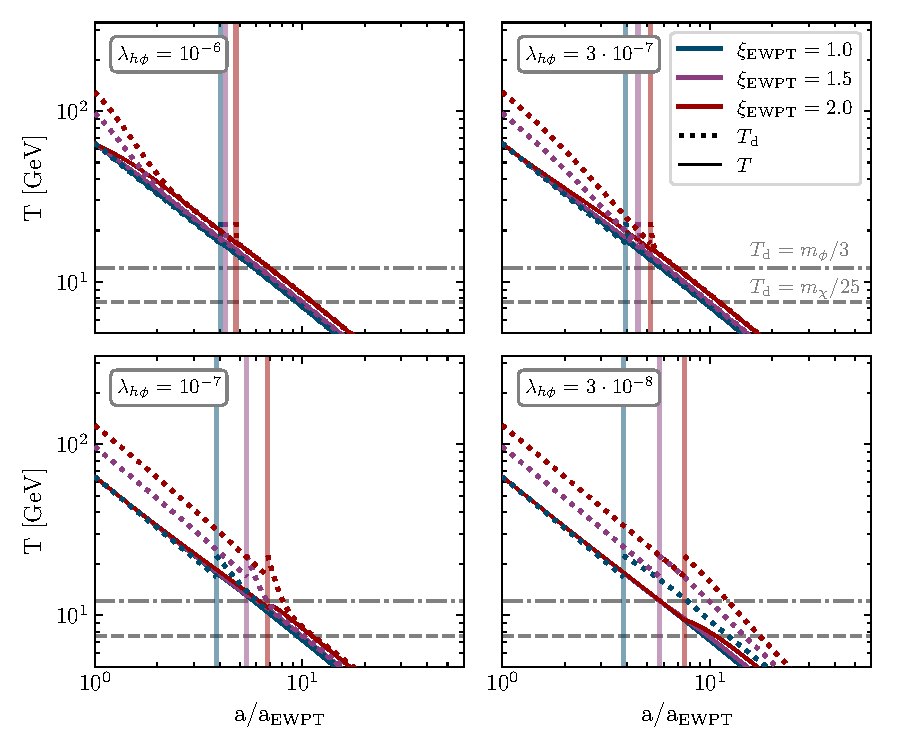
\includegraphics[width=\textwidth]{thesisplots/lisa/thesis_LISA_9}
	\caption{Evolution of the \ac{DS} temperature (dotted) and the \ac{SM} temperature (solid) for different values of the initial temperature ratio $\xi_\EWPT$ as a function of scale factor. The vertical lines indicate the scale factor at percolation, which depends on the temperature ratio. The horizontal lines indicate when the lightest state in the \ac{DS} becomes non-relativistic ($T_\text{d} = m_\phi / 3$) and approximately when the \ac{DM} particles freeze out ($T_\text{d} = m_\chi / 25$). The different panels correspond to different values of the portal coupling $\lambda_{h\phi}$.}
	\label{fig:evolution}
\end{figure}

As discussed above, it is not necessarily the case that the \ac{DS}	is in kinetic equilibrium with the \ac{SM} at high temperatures. In the following, we will therefore take the temperature ratio of the two sectors at the \ac{EWPT}, $\xi_\EWPT$, as a free parameter and calculate the evolution of $\xi$ during the subsequent cosmological stages (see appendix~\ref{app:thermalisation} for details). In fig.~\ref{fig:evolution} we show the visible and \ac{DS} temperatures as a function of the scale factor for different initial values of $\xi_\EWPT$, defined at $T = 150 \, \text{GeV}$. In the four panels \graffito{The portal coupling $\lambda_{h\phi}$ decides on the time of thermalization} the portal coupling was set to the representative values $\lambda_{h\phi} = 10^{-6}$ (top left), $3 \cdot 10^{-7}$ (top right), $10^{-7}$ (bottom left) and $3 \cdot 10^{-8}$ (bottom right). In each panel, we indicate the moment of percolation by a vertical dot-dashed line; the approximate temperature of the dark Higgs becoming non-relativistic ($m_\phi / T_\text{d} = 3$) and the \ac{DM} fermion freezing out ($m_\chi / T_\text{d} = 25$) are indicated by horizontal dotted and dashed lines, respectively. We make the following observations:
\begin{itemize}
	\item For $\lambda_{h\phi} = 10^{-6}$, the two sectors thermalize efficiently already before percolation. The initial value of $\xi_\EWPT$ is therefore inconsequential for the subsequent evolution, and we obtain the same results for all cases.
	\item For $\lambda_{h\phi} = 3 \times 10^{-7}$, the two sectors do exchange energy and entropy already in the unbroken phase, but do not fully thermalize before percolation, such that $\xi_\perc$ depends on $\xi_\EWPT$. After dark symmetry breaking, the two sectors thermalize rapidly, such that the subsequent evolution, and in particular the relic density calculation, do not depend on $\xi_\EWPT$.
	\item For $\lambda_{h\phi} = 10^{-7}$, the energy exchange before dark symmetry breaking is completely negligible. Even after dark symmetry breaking, it will take a while for the temperatures of the two sectors to approach each other. Nevertheless, the two sectors reach equilibrium before the dark Higgs bosons become non-relativistic.
	\item For $\lambda_{h\phi} = 3 \times 10^{-8}$, the two sectors do not quickly thermalize after the \ac{PT}, and the universe enters an early period of cannibal domination.\footnote{For the purpose of this plot, we assume that number-changing processes in the \ac{DS} remain efficient throughout, such that the chemical potential of the dark Higgs boson vanishes and (in the absence of decays) the \ac{DS} temperature grows relative to the \ac{SM} temperature.}
\end{itemize}
In general the value of $\lambda_{h\phi}$ needed to ensure thermalization depends somewhat on the dark Higgs \ac{vev}, since for $m_\phi \ll m_h$ the mixing angle scales as $\theta \propto \lambda_{h\phi} v_{\phi}$. Moreover, for small dark Higgs boson masses, decays into bottom quarks are kinematically forbidden and thermalization is less efficient. For the parameter points that reproduce the observed relic density we find that the \graffito{All considered $\lambda_{h\phi}$ are well bellow direct detection constraints} assumption $\xi = 1$ made in section~\ref{sec:relic} is well justified for $\lambda_{h\phi}$ greater than $10^{-6}$--$10^{-5}$. This value should be compared to the currently strongest bounds from direct detection experiments, which are only sensitive to $\lambda_{h\phi} \gtrsim 10^{-3}$~\cite{Ferber:2023iso}.


\section{Gravitational waves from hot dark sectors}
\label{sec:hot}

While the analysis of the \ac{DSPT} is simplest for $\lambda_{h\phi} > 10^{-6}$, it is phenomenologically interesting to also consider smaller values of $\lambda_{h\phi}$, such that the temperature ratio of the \graffito{Turn up the volume: $\xi_\mathrm{p} > 1$ enhances the \acp{GW}} two sectors before the \ac{PT} may differ from unity. The reason is that $\xi_\perc> 1$ leads to an enhancement of the \ac{GW} signal, as a result of the larger total energy density in the \ac{DS} compared to the \ac{SM} thermal bath~\cite{Breitbach:2018ddu,Ertas:2021xeh}. In this case, however, we also need to consider what happens to the energy density of the \ac{DS} after the \ac{PT}.

If the transfer of energy from the dark to the visible sector after the \ac{PT} is slow, the energy density of the universe will eventually be dominated by non-relativistic \ac{DS} particles. This effect is already visible in fig.~\ref{fig:evolution}, where for small values of
$\lambda_{h\phi} = 3 \times 10^{-8}$ the temperature ratio $\xi$ still differs from unity when the lightest \ac{DS} particle becomes non-relativistic. When the non-relativistic dark Higgs bosons eventually decay into \ac{SM} particles, their entropy is transferred to the thermal bath; this modifies the expansion history of the universe and leads to a dilution of the \ac{GW} signal. It is a-priori unclear whether this dilution effect dominates over \graffito{$\xi_\mathrm{p}$ and $\lambda_{h\phi}$ have competing effects} the enhancement with increasing \ac{DS} temperature, or whether a net increase in the strength of \ac{GW} signals remains. Moreover, the dilution effect also shifts the \ac{GW} frequencies and might thereby spoil the correlation between peak frequency and relic density found in section~\ref{sec:relic}. In the following we will investigate these effects in detail.

If the portal coupling is extremely small, in principle even the relic density calculation could be modified. If the dark Higgs bosons become non-relativistic after freeze-out, in particular, they may come to dominate the energy density of the universe at later times, and dilute not only the \ac{GW} energy density but also the \ac{DM} energy density through their decays (see e.g.~ref.~\cite{Berlin:2016gtr}). If, on the other hand, the dark Higgs bosons are non-relativistic already during freeze-out, inefficient thermalization between the two sectors may additionally \graffito{Other dilution effects} imply a non-trivial evolution of the \ac{DS} temperature during freeze-out. While these are interesting scenarios in their own right, they are beyond the scope of  this thesis. Instead, we will here focus exclusively on the case where the dark Higgs bosons decay sufficiently quickly for the standard freeze-out calculation (with temperature ratio $\xi = 1$) to be valid.

In section~\ref{sec:DSdecaydilution} we introduced the dilution factor $D \equiv S_\mathrm{SM}^{0} / S_\mathrm{tot}^\mathrm{p}$ to account for the dilution of the \ac{GWB}~\cite{Cirelli:2018iax, Ertas:2021xeh}. In fig.~\ref{fig:dilution} we show its dependence on the portal coupling $\lambda_{h\phi}$. Here, we choose the same benchmark point as studied in section~\ref{sec:equilibrium}, and show the result for different values of the initial \ac{DS} temperature ratio $\xi_\EWPT$, defined at $T= 150\,\text{GeV}$. As expected, for sufficiently large $\lambda_{h\phi}$ there is no significant dilution\footnote{In the limit of large portal couplings $\lambda_{h\phi}$, the dilution factor $D$ approaches a value slightly larger than 1. This is an expected feature, indicating a negligible dilution effect that is entirely due to the additional degrees of freedom in the combined thermal bath of \ac{SM} and \ac{DS} particles and not a consequence of additional entropy injection (with respect to $\Lambda$CDM) into the \ac{SM} bath after the \ac{PT}.},  \graffito{Dilution becomes relevant for $\lambda_{h\phi} \ll 10^{-7}$} as entropy is conserved and only relativistic \acp{dof} contribute to the energy content of the universe. However, with decreasing $\lambda_{h\phi}$ this is no longer the case and the dilution factor grows, becoming sizable for $\lambda_{h\phi} \ll 10^{-7}$.

\begin{figure}[t]
	\centering
	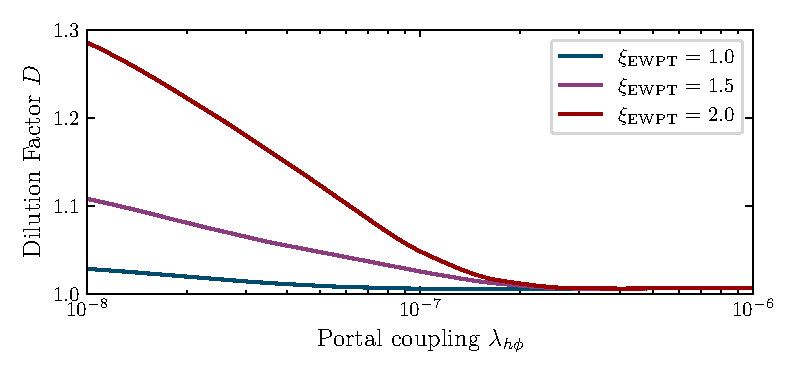
\includegraphics[width=\textwidth]{thesisplots/lisa/thesis_LISA_10}
	\caption{Dilution factor $D$, cf.~eq.~\eqref{eq:dilution}, as a function of the portal coupling $\lambda_{h\phi}$, and for different values of the initial temperature ratio $\xi_\EWPT$ as indicated.
	}
	\label{fig:dilution}
\end{figure}

\begin{figure}[t]
	\centering
	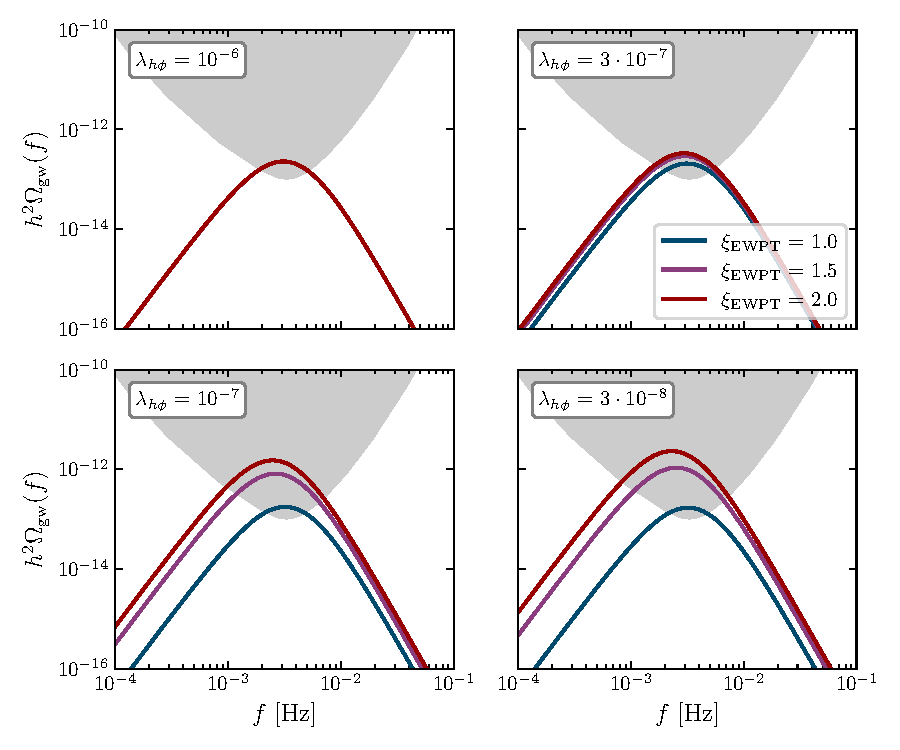
\includegraphics[width=\textwidth]{thesisplots/lisa/thesis_LISA_11}
	\caption{\ac{GW} signal of the scenarios considered in fig.~\ref{fig:evolution}, i.e.~for various values of the portal coupling $\lambda_{h\phi}$ (different panels) and the initial temperature ratio $\xi_\EWPT$ (different colors).}
	%\vspace{-5mm}
	\label{fig:gw_with_xi}
\end{figure}

In fig.~\ref{fig:gw_with_xi} we show the resulting \ac{GW} spectra for $\xi \neq 1$ and $\lambda_{h\phi} < 10^{-6}$. As anticipated, a net enhancement of the \ac{GW} signal is found for $\xi_\EWPT > 1$, provided that $\lambda_{h\phi}$ is sufficiently small for the sectors to not equilibrate before the \ac{PT} (cf.~fig.~\ref{fig:evolution}). The enhancement saturates for $\xi_\EWPT \gtrsim 2$, see also the discussion in ref.~\cite{Ertas:2021xeh}, implying a \ac{DS} energy density that initially \graffito{A net enhancement remains for $\xi_\mathrm{p} > 1$} dominates over that of the \ac{SM} sector. For too small portal couplings $\lambda_{h\phi} \lesssim 3 \times 10^{-8}$, on the other hand, the effect of dilution becomes relevant and the \ac{GW} signal starts to become suppressed. Crucially, changing $\xi$ and $\lambda_{h\phi}$ does not significantly affect the peak frequency, such that the \ac{GW} signal remains within the \ac{LISA} sensitivity range.

\begin{figure}[t]
	\centering 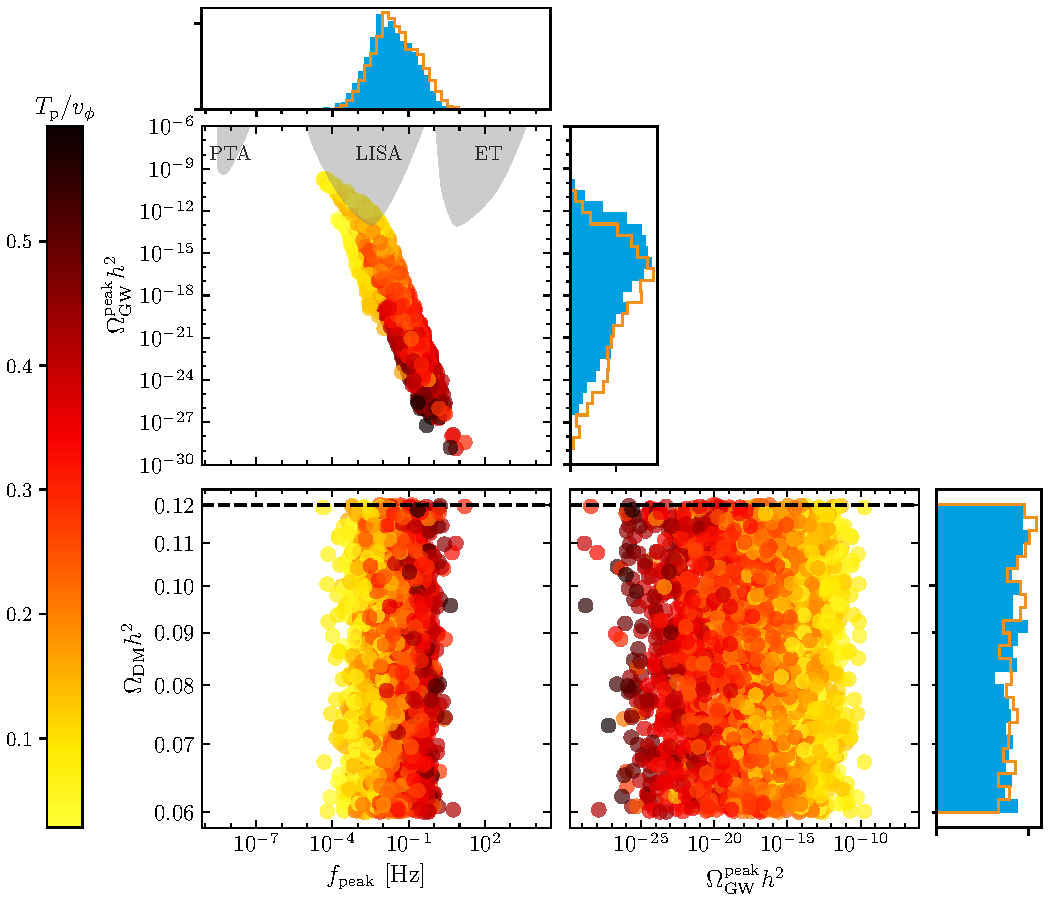
\includegraphics[width=\textwidth]{thesisplots/lisa/thesis_LISA_12}
	\caption{Same as fig.~\ref{fig:triangle-restr}, but without the assumption of thermal equilibrium between the two sectors. Specifically, we consider $\xi_\EWPT = 2$ and $\lambda_{h\phi} = 10^{-7}$. Compared to the situation in fig.~\ref{fig:triangle-restr}  (indicated by the red lines in the 1D histograms), the \ac{GW} amplitude is shifted to slightly larger values, while the peak position remains almost unaffected.}
	\label{fig:triangle-xi2}
\end{figure}

We can now test the robustness of our results from section~\ref{sec:relic}, where we assumed $\xi = 1$ and $\lambda_{h\phi} > 10^{-6}$, by allowing larger values of $\xi$ and smaller values of $\lambda_{h\phi}$. In fig.~\ref{fig:triangle-xi2} we show the same result as in fig.~\ref{fig:triangle-restr}, but now for $\xi_\EWPT = 2$ and $\lambda_{h\phi} = 10^{-7}$. For comparison we show the 1D distributions from fig.~\ref{fig:triangle-restr} as orange lines. In this plot we have removed points for which the \ac{DS} temperature still differs significantly from the \ac{SM} temperature when the dark Higgs boson becomes non-relativistic, i.e.~for which $\xi_\text{nr} > 1.1$ at $T_{\text{d,nr}} = m_\phi / 3$. The reason is that for such cases our final predictions depend on the details of chemical decoupling within the \ac{DS}, which we do not study further \graffito{The correlation is present also when $\xi_\mathrm{EWPT} = 2$ and $\lambda_{h\phi} = 10^{-7}$} in this thesis. While this requirement removes almost half of the parameter points, it does not introduce any significant bias, i.e.~the distributions of $f_\text{peak}$ and $\Omega_\text{GW}^\text{peak} h^2$ look very similar with and without this additional requirement.

The parameter combination $\xi_\EWPT = 2$ and $\lambda_{h\phi} = 10^{-7}$ leads to a nearly maximal enhancement of the \ac{GW} signal. As expected, we find that the peak position of the \ac{GW} signal is not affected, such that the frequency range implied by the observed \ac{DM} relic abundance remains within the \ac{LISA} sensitivity window. The amplitude of the \ac{GW} signal, on the other hand, is slightly enhanced, as can be seen from the comparison in the corresponding one-dimensional histogram. We can make this statement more precise by once again interpreting the density of \graffito{69\% of points with strong supercooling are observable} points in the scatter plots as a probability  distribution for the observables. Compared to fig.~\ref{fig:triangle-restr}, we find that the probability to obtain a signal observable with \ac{LISA} increases from 3\% to 8\%. Limiting ourselves to parameter regions with strong supercooling, the fraction of observable events increases from 35\% to 69\%. We summarize our findings in table~\ref{tab:observable}.


\begin{table}[t]
	\centering
	\begin{tabular}{p{0.48\linewidth}C{0.2\linewidth}C{0.2\linewidth}}
		\toprule
		& \multicolumn{2}{c}{\centering \textbf{Observable by \ac{LISA}}} \\
		\textbf{Selection requirement} & $\xi_\text{EWPT} \!=\! 1$, $\lambda_{h\phi} \!=\!  10^{-6}$ & $\xi_\text{EWPT} \!=\!  2$, $\lambda_{h\phi} \!=\!  10^{-7}$ \\
		\midrule
		Full sample & 0.1\% & 0.5\% \\[1ex]
		\ac{FOPT} & 0.8\% & 3\% \\
		\ac{FOPT} + relic density & 3\% & 8\% \\[1ex]
		Strong supercooling & 10\% & 21\% \\
		Strong supercooling + relic density & 35\% & 69\% \\
		\bottomrule
	\end{tabular}
	\caption{Fraction of parameter points that predict an observable \ac{GW} signal for \ac{LISA} after imposing various selection requirements on the sample of points drawn from the parameter ranges discussed in section~\ref{sec:GWspec}.}
	\label{tab:observable}
\end{table}

We emphasize that this large increase is a result of fixing $\xi$ and $\lambda_{h\phi}$ to particular values. If we instead vary $\xi$ and $\lambda_{h\phi}$ as part of the scan, most parameter combinations will either give very similar results to the case $\xi = 1$ considered in section~\ref{sec:relic} or lead to an extended period where the \ac{DS} energy density dominates.

\section{Conclusions}
\label{sec:conclusions}

In this chapter we explored correlations between the \ac{DM} relic density and \ac{GW} signals arising from a \ac{FOPT} that breaks a $U(1)'$ gauge symmetry and gives rise to the mass of a fermionic \ac{DM} particle. We demonstrated that, while the amplitude of the \ac{GW} signal depends on the details of the effective \graffito{A \ac{FOPT}-triggered freeze-out hints towards \ac{LISA} frequencies} potential and can vary over many orders of magnitude, the peak frequency is tightly constrained once we impose the observed value for the \ac{DM} relic abundance. Intriguingly, the peak frequency is found to lie exactly in the milli-Hertz range, which will be explored by the \ac{LISA} mission.

The \ac{DS} considered in this chapter is characterized by four parameters: the dark gauge coupling $g$, the quartic coupling of the dark Higgs field $\lambda$, the dark Yukawa coupling $y$ and the dark Higgs \ac{vev} $v_\phi$. As a first step, we calculated the effective potential and the percolation temperature of the \ac{PT} and identified the regions of parameter space that give a strong (large $\alpha$) and not too fast ($\beta/H\sim10^2$--$10^4$) \ac{PT}, corresponding to potentially observable \ac{GW} signals. We showed in particular that large \ac{GW} signals require sizable couplings $g$ and $\lambda$ and occur also for large values of $y$.
%
The relic density of the \ac{DS} is determined by annihilations of \ac{DM} fermions into pairs of dark Higgs bosons. The requirement to match the observed \ac{DM} relic density then requires that the \ac{DM} fermion cannot be much lighter than the dark Higgs boson, with mass $m_\phi\sim v_\phi$, which in turn implies a sizable Yukawa coupling and a \ac{DM} mass that is comparable to the dark Higgs \ac{vev} $v_\phi$. The dark Higgs \ac{vev}, on the other hand, \graffito{The correlation is due to requiring a strong \ac{FOPT} \& imposing $\Omega_\mathrm{DM} h^2 = 0.12$} determines the percolation temperature and hence the peak frequency of the resulting \ac{GW} signal. This connection leads to a tight correlation between relic density and \ac{GW} peak frequency. Through comprehensive scans of the parameter space, we confirmed that this correlation is indeed highly generic in our model.

A rigorous statistical interpretation of our results is beyond the scope of this chapter, but some estimates of the significance of the samples can be performed. A rough measure of the fine-tuning required to have a visible signal at \ac{LISA} can be obtained by assuming that  \graffito{A \ac{FOPT} producing relic \ac{DM} is observable with 35\% chance} the sampling distributions of the parameters act as prior probabilities, and that the sampling density of points hence indicates the posterior distributions of derived quantities. Indeed, the majority of points drawn from these distributions do not feature any \ac{FOPT} at all. Out of the points that feature a strongly-supercooled \ac{PT} ($T_\perc / T_\crit < 0.5$), the probability of producing a visible signal at \ac{LISA} in our model is around 10\%. With the additional requirement that the observed \ac{DM} relic abundance be reproduced, this probability increases to 35\%, as a result of the strong correlation between the predicted relic density and the peak frequency of the \ac{GW} signal (see fig.~\ref{fig:triangle-restr}).

We then studied two connected questions: How does the \ac{DS} transfer its energy density to the \ac{SM}? And is it justified to assume the same temperature for both sectors? Indeed, the \ac{PT} leads to an increase of the \ac{DS} temperature, as vacuum
energy is converted into rest mass and kinetic energy. Having confirmed that the \ac{DS} itself thermalizes immediately after the \ac{PT}, we discussed in detail how the two sectors thermalize with \graffito{\ac{DS} thermalization is efficient} each other for the specific case that the two Higgs bosons in the theory interact via the portal coupling $\lambda_{h\phi}$. After both electroweak symmetry breaking and \ac{DS} symmetry breaking, this interaction leads to mixing between the Higgs bosons, such that they can decay into each other as well as into fermions of both sectors.

We derived and solved the Boltzmann equations for the entropy transfer between the two sectors and showed that for $\lambda_{h\phi} > 10^{-6}$ the assumption of equal temperature for both sectors is well justified. This portal coupling is small enough to be consistent with all laboratory constraints, in particular with direct detection experiments. For even smaller portal couplings, on the other hand, the temperatures of the two sectors may differ significantly, motivating us to consider the initial temperature ratio $\xi_\EWPT$ as a free parameter. While small values of $\lambda_{h\phi}$ combined with large initial values of $\xi_\EWPT$ may lead to an increase in the amplitude of the \ac{GW} signal, the dark Higgs bosons will decay \graffito{For $\lambda_{h\phi} \approx 10^{-7}$, $\xi > 1$ leads to stronger \acp{GW}} only slowly after the \ac{PT} and may end up dominating the energy density of the universe. The resulting entropy injection would then lead to a substantial dilution of \ac{GW} signals. We find that for $\lambda_{h\phi} \approx 10^{-7}$ a net enhancement remains, demonstrating that it is possible to have $\xi > 1$ during the \ac{DSPT} while at the same time avoiding the dilution of the \ac{DS} signal due to sufficiently rapid thermalization afterwards. Repeating our parameter scans for $\xi = 2$ and $\lambda_{h\phi} = 10^{-7}$, we find that the impact on the \ac{GW} spectrum is only modest; while the typical amplitude is slightly enhanced, the peak frequency remains unchanged. In combination, these effects increase the fraction of points with a strongly supercooled  \ac{PT} that would be observable in \ac{LISA} to 69\%. Hence, our conclusion regarding the correlation between the \ac{DM} relic abundance and the \ac{GW} peak frequency applies also to \acp{DS} that thermalize only slowly with the \ac{SM}.

An interesting open question is how the relic density calculation would change for even smaller values of the portal coupling than what we consider. In this case, the energy density of the universe would be dominated by non-relativistic dark Higgs bosons, which may develop a chemical potential if number-changing processes are inefficient. The relic density calculation then requires solving a coupled set of Boltzmann equations with non-trivial evolution of the \ac{DS} temperature. While the details of this calculation are beyond the scope of this thesis, the general expectation is that the \ac{DM} relic abundance \graffito{Can chemical potentials push the signal to nHz?} would be increased. This might open up the possibility to have a \ac{DSPT} in the nano-Hertz frequency range and hence of interest in the context of recent results from \acp{PTA}~\cite{NANOGrav:2023gor, EPTA:2023fyk, Reardon:2023gzh}. Another promising avenue for further investigations opens up due to our findings regarding the bubble wall velocity presented in appendix~\ref{app:darkwalls}. There exists a potentially relevant part in the parameter space of our model in which the 
Bödeker-Moore criterion hints towards non-relativistic bubble wall velocities. For such low wall speeds the effect of bubble 
filtering~\cite{Baker:2019ndr} may be non-negligible, and the calculation of the \ac{DM} relic abundance is expected to be more involved than presented here.

Let us finally mention that even for tiny portal couplings there is a chance to actually detect the \ac{DM} particles that we consider: unlike for annihilation into dark Higgs boson pairs, the mixed annihilation channel into one dark Higgs boson and one dark photon is not suppressed in the limit of small \ac{DM} velocities. If kinematically allowed, it \graffito{Indirect detection probes} may thus lead to observable signals in indirect detection experiments~\cite{Bell:2016fqf} such as CTA~\cite{CTA:2020qlo}. Such an observation would raise the possibility to explore in practice the correlations studied in this chapter and pin down the detailed structure of the \ac{DS}.


\newpage

\appendix
\section{Dark bubble walls}
\label{app:darkwalls}

In addition to the strength $\alpha$ of the \ac{PT}, its speed $\beta/H$, the percolation temperature $T_\perc$, and the temperature ratio $\xi_\perc$, it is also necessary to know the speed of the bubble walls $\vw$ in order to determine the processes that dominate the \ac{GW} signal from a \ac{DSPT}. While the former parameters can be obtained from the effective potential $V_\text{eff}(\phi, T_\text{d})$, the bubble wall velocity depends on plasma effects of the expanding bubble walls and therefore requires additional considerations. For bubbles expanding into the vacuum (i.e.~if bubbles expand into a plasma that is not influenced by a change of the scalar \ac{vev}), there is no source of friction, such that bubble walls can accelerate up to the point of \graffito{The dark wall velocity} their collision. For walls that interact with the surrounding plasma, on the other hand, several model-dependent sources of friction have been discussed~\cite{Liu:1992tn, Bodeker:2009qy, Bodeker:2017cim, Azatov:2020ufh, GarciaGarcia:2022yqb}. If the friction increases with the bubble wall velocity, the acceleration of the bubble walls eventually stalls and a terminal velocity
is reached. In this case, the bulk motion of the plasma dominates the \ac{GW} spectrum~\cite{Azatov:2023xem}.

In this paper we take the approach suggested in ref.~\cite{Vanvlasselaer:2022fqf}, i.e.~we show that $\vw$ is either expected to be non-relativistic in our model or that the bubbles are \graffito{Gauge bosons prohibit runaway} relativistic, but do not run away due to the emission of soft gauge bosons in the bubble walls. We conclude that the plasma motion is responsible for the dominant part of the \ac{GW} signal and the contribution from bubble wall collisions is negligible.

To decide whether a bubble wall can accelerate up to \graffito{The Bödeker-Moore criterion} relativistic velocities, we use the Bödeker-Moore criterion~\cite{Bodeker:2009qy}, which relates the velocity-independent \acf{LO} bubble wall friction $\mathcal{P}_\mathrm{LO}$ to the amount of liberated vacuum
energy density $\Delta V_\text{eff}$:
\begin{align}
	\text{BM criterion:} \quad \begin{cases}
		\Delta V_\text{eff} > \mathcal{P}_\mathrm{LO} \quad \text{Relativistic bubble walls.} \\
		\Delta V_\text{eff} < \mathcal{P}_\mathrm{LO} \quad \text{Non-relativistic bubble walls.} \label{eq:Bodeker}
	\end{cases}
\end{align}
We emphasize that this criterion is insufficient to decide whether walls can run away (i.e.~accelerate indefinitely), because of the \ac{NLO} friction $\mathcal{P}_\mathrm{NLO}$, which scales with powers of $\gamma_\text{w} = 1/\sqrt{1 - \vw^2}$~\cite{Bodeker:2017cim,Hoche:2020ysm,Gouttenoire:2021kjv}. Bubbles can run away only if $\Delta V_\text{eff} > \mathcal{P}_\mathrm{LO} + \mathcal{P}_\mathrm{NLO}$ for all $\vw$. Otherwise they will reach a relativistic terminal velocity given by the equilibrium of forces, $\Delta V_\text{eff} = \mathcal{P}_\mathrm{LO} + \mathcal{P}_\mathrm{NLO}$.

The \ac{LO} friction due to particles acquiring a mass when crossing the bubble wall is given
by~\cite{Bodeker:2009qy, Espinosa:2010hh}
\begin{align}
	\mathcal{P}_\mathrm{LO} \simeq \sum_i g_i \, c_i \frac{\Delta m_i^2}{24} T_\text{d,p}^2 \,, \label{eq:LOfriction}
\end{align}
where $\Delta m_i^2$ is the positive \graffito{\ac{LO} friction from mass increase $\Delta m_i^2$} change of the mass square of particle species $i$ during the \ac{PT}, $g_i$ is the corresponding number of degrees of freedom, and $c_i = 1$ $(1/2)$ for bosons (fermions). This expression assumes that the particle masses outside the bubble are below the \ac{DS} temperature. For ultra-relativistic bubble walls, the production of heavy particles with mass up to $\gamma_\text{w} T_\text{d,p}$ can also add to the \ac{LO} friction~\cite{Azatov:2020ufh}. For the \ac{DS} considered in this chapter, all particles are light before the \ac{PT} and subsequently obtain a mass comparable to the scale of the \ac{PT}, such that \eqref{eq:LOfriction} is the only relevant contribution to the \ac{LO} friction.

In the case of a broken $U(1)'$ with a fermionic species, the \ac{LO} friction reads~\cite{Espinosa:2010hh}
\begin{align}
	\mathcal{P}_\text{LO} \simeq \left(3 m_{A'}^2 + m_\phi^2 + 2 m_\chi^2\right) \, \frac{{T_{\text{d,p}}}^2}{24} \approx \frac{m_{A'}^2 \, {T_{\text{d,p}}}^2}{8} \,,
\end{align}
where in the last step we have used that the dominant contribution comes from the heaviest state in the \ac{DS}, which in the parameter regions of interest is the dark photon. The amount of released vacuum energy $\Delta V_\text{eff}$ can be estimated from the zero-temperature potential, which gives
\begin{align}
	\Delta V_\text{eff} \approx \frac{\lambda}{4} v_\phi^4 = \frac{m_\phi^2}{8} v_\phi^2 \,.
\end{align}
Hence we find that the Bödeker-Moore criterion for relativistic bubble walls is satisfied if $m_\phi / m_{A'} > {T_{\text{d,p}}} / v_\phi$, which is the case for the parameter regions that give strongly supercooled \acp{PT} corresponding to observable \ac{GW} signals ($T_{\text{d,p}} \lesssim 0.1 \, v_\phi$). In these parameter regions, \graffito{Strong supercooling implies fast walls} the bubble walls are therefore expected to be relativistic, $\vw \rightarrow 1$. This finding also implies that we can neglect the effect of bubble filtering, which is only relevant in the (deeply) non-relativistic regime $\vw \ll 1$~\cite{Baker:2019ndr,Chway:2019kft}. In the regions in which weaker \ac{GW} signals are expected, the Bödeker-Moore criterion instead hints towards slower bubble walls, see fig.~\ref{fig:verifyvw}.

The \ac{NLO} friction created by the emission of soft dark photons into the broken phase quickly starts to grow with $\gamma_\text{w}$. The bubble walls will therefore reach a terminal, asymptotic bubble wall velocity which is close to the speed of light. The precise value of $\gamma_\text{w}^\text{terminal}$ is unnecessary for our purposes, as the existence of a terminal yet relativistic bubble wall velocity is sufficient to assume a dominant \ac{GW} emission through bulk fluid motion. \graffito{Sound waves are dominant \ac{GW} source} A more refined calculation of the respective energy budgets for the processes emitting gravitational radiation was performed
in refs.~\cite{Lewicki:2022pdb,Ellis:2020nnr, Ellis:2019oqb}. In ref.~\cite{Lewicki:2022pdb} it was shown that for sufficiently high terminal bubble wall velocities the fluid profiles are strongly peaked, such that the emitted \ac{GW} spectral shapes are in fact indistinguishable from bubble collisions. We conclude that it is hence a reasonable approximation to work with a \ac{GW} spectrum that is solely sourced through sound waves.

\begin{figure}[t]
	\centering
	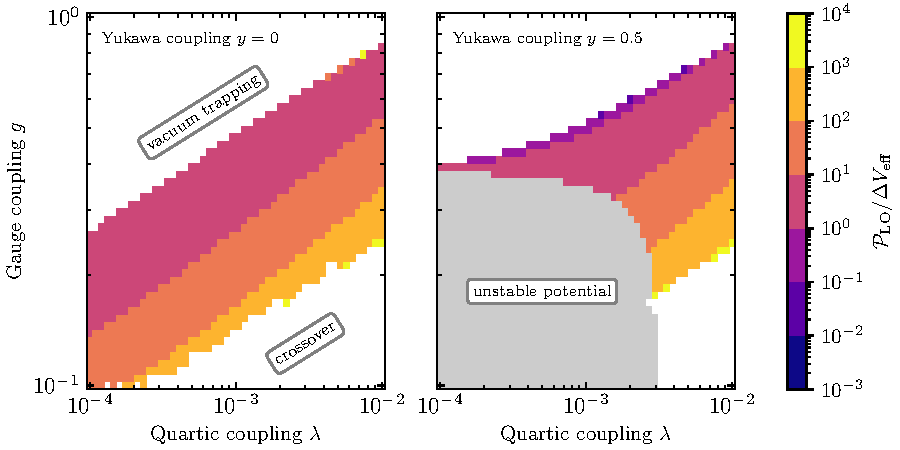
\includegraphics[width=\linewidth]{thesisplots/lisa/thesis_LISA_13}
	\caption{The leading-order friction $\mathcal{P}_\text{LO}$ over the difference $\Delta V_\text{eff}$ in potential energy between the true and false vacuum phases as a function of the quartic coupling $\lambda$ and the gauge coupling $g$ for values of the Yukawa coupling $y = 0$ and $y = 0.5$. Values greater than one indicate that relativistic bubble wall velocities cannot be reached, cf.~eq.~\eqref{eq:Bodeker}. For values smaller than one, a relativistic terminal velocity is expected.}
	\label{fig:verifyvw}
\end{figure}

\section{Detail on thermalization and freeze-out}
\label{app:thermalisation}

Here we discuss the processes we consider for the entropy transfer between the \ac{DS} and the \ac{SM}.

\subsection{The thermal mixing angle}

The Higgs mixing angle defined in eq.~\eqref{eq:mixing-angle} depends on temperature through the masses and \acp{vev} of the two Higgs bosons. The temperature dependence of the dark Higgs boson can be directly obtained from the effective potential, whereas we follow ref.~\cite{Bringmann:2021sth} to implement the \graffito{Mixing depends on temperature} temperature dependence of the \ac{SM} Higgs boson. For large values of the dark Higgs \ac{vev}, we sometimes encounter the situation that the \ac{SM} Higgs and dark Higgs mass become similar or even cross, in which case the mixing angle apparently diverges. To regulate this unphysical divergence, we have to include the finite width $\Gamma_{h}$ of the Higgs resonance. As shown in ref.~\cite{Fradette:2018hhl}, including the width leads to an effective mixing angle given by 
\begin{align}
	\theta_{\mathrm{eff}}^2(T) = \frac{\left(\lambda_{h\phi} v_{h}(T)v_{\phi}(T) \right)^2}{(m_{\phi}^2(T) -
		m_{h}^2(T))^2 + (m_{\phi}(T)\Gamma_{h})^2} \,.
\end{align}


\subsection{The Boltzmann equation for entropy transfer}

In our analysis we specify the initial conditions, i.e.~the temperature ratio $\xi_\EWPT$ of the \ac{DS} and \ac{SM} bath at the \ac{EWPT}, for which we take $T_\EWPT = 150\,\text{GeV}$. \graffito{On the order of \ac{DSPT} and \ac{EWPT}} Which processes contribute to the thermalization of the two sectors depends on whether or not the $U(1)'$ gauge symmetry is already broken at this point. We consider two different timelines:
\begin{itemize}
	\item The electroweak symmetry breaks before the \ac{DSPT}. This is the case for the majority of our parameter space. Here, the thermalization between the two sectors is initially determined by the processes $h h \leftrightarrow \Phi\Phi$ and the decay of the \ac{SM} Higgs $h \rightarrow \Phi\Phi$. Additional processes can only contribute after the \ac{DSPT}.
	\item The \ac{DSPT} occurs before the \ac{EWPT}. This can happen for parameter points with a large \ac{vev} of the dark Higgs and not too strong supercooling. Once both symmetries are broken, thermalization proceeds via $hh \leftrightarrow \phi\phi$, the decays of the \ac{SM} Higgs into dark Higgs $h \rightarrow \phi\phi$ if it is kinematically allowed, and the decays of the dark Higgs into \ac{SM} particles $\phi \rightarrow \mathrm{SM} \ \mathrm{SM}$ through Higgs mixing.
\end{itemize}
In the following we give the relevant expressions contributing to the entropy transfer.

\paragraph{$2\to 2$ processes}
\label{subsec:2to2processes}

In most regions of parameter space, the \ac{DS} phase is unbroken immediately after the \ac{EWPT}, such that there are no dark Higgs boson decays that can transfer entropy between the two sectors. Here the $2 \to 2 $ process induced by the portal coupling $\Phi\Phi \leftrightarrow hh$ become relevant. Since the particles' \graffito{Thermalization through $\Phi\Phi \leftrightarrow hh$} thermal masses are smaller than the temperature, we cannot take the usual non-relativistic approach. Instead we will follow the relativistic treatment of the calculation of the entropy transfer developed in refs.~\cite{Arcadi:2019oxh,DeRomeri:2020wng}, which we briefly sketch here. The heat transfer for $2\to2$ processes can be expressed as 
\begin{align}\label{eq:entropy-22}
	\dot{q}\big|_{2\to2}^\DS 
	&= \int \frac{\dd^3p_1}{(2\pi)^{3}}\frac{\dd^3p_2}{(2\pi)^{3}2E_{2}}\frac{\dd^3k_1}{(2\pi)^{3}2E_{k_{1}}}
	\frac{\dd^3k_2}{(2\pi)^{3}2E_{k_{2}}} |\mathcal{M}|^2 (2\pi)^4\delta(\Sigma p) \nonumber \\
	& ~~~~~~~~~~~~~~~~~~~~~~~~~~~~~~\times f(p_{1})f(p_2)(1+ f(k_{1}) (1+f(k_2)) \nonumber\\
	&= \int \frac{\dd^3p_1}{(2\pi)^{3}2E_{1}}\frac{\dd^3p_2}{(2\pi)^{3}2E_{2}} 8 E_{1} F(p_1, p_2) \sigma(p_1, p_2) f(p_1) f(p_2)\,.
\end{align}
Here the final state statistical factors are absorbed into the cross section and $F(p_{1}, p_{2}) = \sqrt{(p_1\cdot p_2)^2-m^2_{1}m_2^2}$. It is easiest to calculate this cross section in the center of mass frame. However, since the Bose-Einstein and Fermi-Dirac distributions are not Lorentz-invariant we have to apply a Lorentz boost $\Lambda$ from the cosmic rest frame where $u = (1, 0, 0, 0)^{T}$ into the center of mass frame, which can be parameterized by the rapidity $\eta$ and two angles $\theta$ and $\varphi$; for details see ref.~\cite{Arcadi:2019oxh}. The phase space distribution becomes
\begin{align}
	f(k) = \frac{1}{e^{u \cdot k/T_\text{d}} \mp 1} \overset{\Lambda}{\rightarrow} f_{\Lambda}(k) =
	\frac{1}{e^{\left( k_{0} \cosh\eta + k_{1}\sinh\eta  \right)/T_\text{d} }\mp 1}\,.
\end{align}
With this, we can rewrite the center of mass cross section as
\begin{align}
	\sigma_{\mathrm{CM}}(p_1,p_2) &= \frac{1}{(2\pi)^216F(p_1,p_2)}  \int \dd \varphi \, \dd \cos\theta \left| \mathcal{M} \right|^2 \nonumber \\ & \qquad \qquad  \times 
	\frac{\sqrt{E^2-m_{f}^2}}{E} \left( (1+f_{\Lambda}(k_1))(1+ f_{\Lambda}(k_2)) \right)\,.
\end{align}
The matrix element for the processes $\Phi\Phi\to hh$ is at tree level simply given by $\mathcal{M} = i\lambda_{h\phi}$. For this angle-independent transition amplitude, we can integrate over the solid angle and obtain
\begin{align}
	\sigma_{\mathrm{CM}} &= \frac{|\mathcal{M}|^2}{64\pi E^2} \frac{T_\text{d}}{\sqrt{E^2-m_{\Phi}^2} \sinh{\eta}}
	\frac{1}{1-e^{- \frac{2E}{T_\text{d}}\cosh\eta}} \nonumber \\ & \quad \times  \ln \underbrace{\left[ \frac{\sinh \left( \frac{E\cosh\eta +
				\sqrt{E^2-m_{h}^2}\sinh\eta}{2T_\text{d}} \right)}{\sinh \left( \frac{E\cosh\eta -
				\sqrt{E^2-m_{h}^2}\sinh\eta}{2T_\text{d}} \right)} \right]}_{\equiv \lambda(E, \eta, T_\text{d}, m_{h})} \, .
\end{align}
In the case of initial and final states with respectively equal masses, eq.~\eqref{eq:entropy-22} reduces to
\begin{align}
	I_{\Phi\Phi \rightarrow h h}  &\equiv \frac{2T_{\mathrm{d}}}{\pi^4} \int_{m_{\Phi}(T_\text{d})}^{\infty}\diff E \sqrt{E^2-m_{\Phi}^2}E^4  \nonumber \\ & \qquad \qquad \times 
	\int_{0}^{\infty}\diff \eta \frac{\sigma_{\mathrm{CM}}  \sinh\eta\cosh\eta}{e^{2E\cosh\eta/T_{\mathrm{d}}}-1}
	\ln \lambda(E, \eta, T_\mathrm{d}, m_{\Phi}) \, .% (E,\eta, T_\mathrm{SM}) 
\end{align}
This expression can now be efficiently evaluated numerically. An analogous expression is obtained for the process $h h \rightarrow \phi \phi$.

We note that in principle there are additional $2 \to 2$ processes that may contribute to thermalization. The process $\phi \phi \to t \bar{t}$ via an off-shell SM Higgs boson is strongly Boltzmann-suppressed below the \ac{EWPT}~\cite{Bringmann:2021sth} and does not give a relevant contribution in the temperature range that \graffito{We neglect $\phi + q \to g + q$} we consider. However, processes such as $\phi + q \to g + q$ with a quark in the $t$-channel can give a relevant contribution if the decay $\phi \to b \bar{b}$ is kinematically forbidden~\cite{Evans:2017kti,Fradette:2018hhl}. Since this is the case only in a very small fraction of the parameter space that we consider, we neglect these processes, thus giving a conservative estimate of the thermalization rate.

\paragraph{Standard Model Higgs boson decays}
\label{app:inverse-SM-Higgs-decays}

After both symmetries are broken and for temperatures comparable to the \ac{SM} Higgs boson mass, a second process of interest besides dark Higgs decays is the resonantly enhanced pair-annihilation of dark Higgs bosons into predominantly bottom quarks: $\phi \phi \to h \to b \bar{b}$. In thermal equilibrium, the rate of this process can be related to the inverse process, which is the decay $h \to \phi \phi$ with partial width given by
\begin{align}
	\Gamma_{h\to\phi\phi} &= \frac{(m_h^2 + 2 m_\phi^2)^2 \, \sin^2 2 \theta_{\mathrm{eff}}}{128 \pi \, m_h}
	\left(1 - \frac{4 m_\phi^2}{m_h^2}\right)^{1/2} \nonumber \\ & \quad \times \left(\frac{1}{v_\phi} \cos \theta_{\mathrm{eff}}
	+ \frac{1}{v_h} \sin \theta_{\mathrm{eff}} \right)^2 \,.
\end{align}
This gives the additional term in the heat transfer rate
\begin{align}
	\dot{q}\big|_{h\to\phi\phi}^\DS =  - m_{h}\Gamma_{h \to \phi \phi} n^\text{eq}_h
	\left[ 1 - \left(\frac{n_\phi}{n^\text{eq}_\phi}\right)^2 \right]\,.
\end{align}
Before the \ac{DSPT}, we also have the decay $h \rightarrow \Phi\Phi$ with the decay rate
\begin{align}
	\Gamma_{h\to\Phi\Phi} = \frac{\lambda_{h\phi}^2 v_{h}^{2}}{128 \pi \, m_h} \,,
\end{align}
which can be treated in analogy to the case above.

\paragraph{Full Boltzmann equation}

The full Boltzmann equation that we solve before the \ac{PT}, in case \graffito{Before the \ac{DSPT}, after the \ac{EWPT}} it occurs after the \ac{EWPT} then reads
\begin{align}
	\dot{s}_{\mathrm{DS}} + 3H s_{\mathrm{DS}} &= - \frac{m_h}{T_{\mathrm{d}}}\Gamma_{h\rightarrow\Phi\Phi} n_{h}^{\mathrm{eq}}
	\left[\left(\frac{n_{\phi}}{n_{\phi}^{\mathrm{eq}}}  \right)^2 - 1  \right] \nonumber \\ & \quad 
	- \frac{1}{T_{\mathrm{d}}} I_{\Phi\Phi\to hh}
	% (T_{\mathrm{DS}}, m_{\Phi}^{T_{\mathrm{DS}}}, T_{\mathrm{SM}}, m_{H}^{T_{\mathrm{SM}}})
	+ \frac{1}{T_{\mathrm{d}}}I_{hh\to \Phi\Phi} \,. 
	%(T_{\mathrm{SM}}, m_{H}^{T_{\mathrm{SM}}}, T_{\mathrm{DS}}, m_{\Phi}^{T_{\mathrm{DS}}})
\end{align}
The equation for the case of the \ac{DSPT} occurring before the \ac{EWPT} follows analogously. \graffito{After both \acp{PT}} After both symmetries are broken the full Boltzmann equation reads 
\begin{align}
	\dot{s}_{\mathrm{DS}} + 3H s_{\mathrm{DS}}
	&= - \frac{m_\phi}{T_\mathrm{d}}\Gamma_{\phi \to \mathrm{SM}\mathrm{SM}} n^\text{eq}_\phi
	\left( \frac{n_\phi}{n^\text{eq}_\phi} - 1 \right) \nonumber \\ & \quad 
	+ \frac{m_{h}}{T_\mathrm{d}}\Gamma_{h \to \phi \phi} n^\text{eq}_h
	\left[ 1 - \left(\frac{n_\phi}{n^\text{eq}_\phi}\right)^2 \right] \notag\\
	& \quad - \frac{1}{T_{\mathrm{d}}} I_{\phi\phi\to hh} + \frac{1}{T_{\mathrm{d}}}I_{hh\to \phi\phi} \,.
\end{align}
where we use the decay widths of the \ac{SM} Higgs into other \ac{SM} particle pairs from ref.~\cite{Ferber:2023iso}. The equations for the \ac{SM} entropy follow analogously.

\subsection{Annihilation cross sections}
\label{app:annihilation}

In the following we list the various \ac{DM} annihilation cross sections in the non-relativistic limit, up to second order in the center-of-mass velocity $v$ (of each of the \ac{DM} particles):
\begin{align}\label{eq:sig-cc-aa}
	(\sigma v)_{\chi\chi \to A^{\prime}A^{\prime}}
	= &   \frac{m_{A'}^4 (m_\chi^2 - m_{A'}^2)^{3/2}}{64 \pi \, v_\phi^4 \, m_\chi(m_{A'}^2 - 2 m_\chi^2)^2} \nonumber \\ & +
	\frac{v^2 \sqrt{m_\chi^2 - m_{A'}^2}}{384 \pi \, v_\phi^4 \, m_\chi (m_\phi^2 - 4 m_\chi^2)^2 (m_{A'}^2 - 2 m_\chi^2)^4} \nonumber \\ & \quad \times
	\Big[144 m_{A'}^{12} m_\chi^2   \nonumber \\ & \qquad 
	+ 2 m_{A'}^{10} (7 m_\phi^4 - 88 m_\phi^2 m_\chi^2 - 432 m_\chi^4)  \nonumber \\ & \qquad 
	+ 128 m_\chi^{10} (m_\phi^4 + 8 m_\chi^4) \nonumber \\ & \qquad  -	64 m_{A'}^2 m_\chi^8 (3 m_\phi^4 + 16 m_\phi^2 m_\chi^2 +
	32 m_\chi^4) \nonumber \\ & \qquad 
	+ 4 m_{A'}^4 m_\chi^6 (17 m_\phi^4 + 600 m_\phi^2 m_\chi^2 + 592 m_\chi^4) \nonumber \\ & \qquad +
	m_{A'}^8 (-73 m_\phi^4 m_\chi^2 + 1128 m_\phi^2 m_\chi^4 + 1840 m_\chi^6) \nonumber \\ & \qquad + 4 m_{A'}^6 (25 m_\phi^4 m_\chi^4 -
	648 m_\phi^2 m_\chi^6 - 496 m_\chi^8)\Big]\nonumber \\
	&+ \mathcal{O}\left(v^4\right)
\end{align}
\begin{align}
	(\sigma v)_{\chi\chi \to \phi\phi}
	= & \frac{v^2 m_\chi \sqrt{m_\chi^2 - m_\phi^2} \left(3 m_\phi^4 - 8 m_\phi^2 m_\chi^2 + 8 m_\chi^4\right)}{192 \pi \, v_\phi^4 (m_\phi^2 - 4 m_\chi^2)^2 (m_\phi^2 - 2 m_\chi^2)^4}  \nonumber \\ & \quad \times  \small(9m_\phi^8 - 64 m_\phi^6 m_\chi^2 + 200 m_\phi^4 m_\chi^4  \nonumber \\ & \qquad - 352 m_\phi^2 m_\chi^6 + 288 m_\chi^8\small) \nonumber\\
	& + \mathcal{O}\left(v^4\right)
\end{align}
%\newpage
\begin{align}
	(\sigma v)_{\chi\chi\to A^{\prime}\phi}
	= & \frac{1}{2048 \pi v^4 m_\chi^4} \nonumber \\
	& \quad \times (m_{A'}^4 - 2m_{A'}^2m_\phi^2 + m_\phi^4 -
	8m_{A'}^2m_\chi^2 \nonumber \\
	& \qquad - 8m_\phi^2m_\chi^2 + 16m_\chi^4)^{3/2} \nonumber \\
	& + \frac{v^2 \sqrt{m_{A'}^4 + (m_\phi^2 - 4m_\chi^2)^2 -
			2m_{A'}^2(m_\phi^2 + 4m_\chi^2)}}{12288 \pi \, v_\phi^4 m_\chi^4 (m_{A'}^2 - 4m_\chi^2)^2  (m_{A'}^2 + m_\phi^2 - 4m_\chi^2)^4} \nonumber \\ & \quad \times
	\Big[ -11m_{A'}^{16}  - 2m_{A'}^{14}(11m_\phi^2 - 228m_\chi^2) 
	\nonumber \\ & \qquad 
	- 16m_\chi^4(m_\phi^2 - 4m_\chi^2)^4 \nonumber \\ & \qquad \quad \times
	(15m_\phi^4 - 80m_\phi^2m_\chi^2 +
	16m_\chi^4) \nonumber \\ & \qquad
	- m_{A'}^{12}(-11m_\phi^4 -
	1200m_\phi^2m_\chi^2 + 7264m_\chi^4)
	\nonumber \\ & \qquad +
	4m_{A'}^{10}(11m_\phi^6 +
	266m_\phi^4m_\chi^2  \nonumber \\ & \qquad \quad -
	4328m_\phi^2m_\chi^4 + 15136m_\chi^6) \nonumber \\ & \qquad +
	8m_{A'}^2m_\chi^2
	(m_\phi^2 - 4m_\chi^2)^2  \nonumber \\ & \qquad \quad \times
	(15m_\phi^8 - 244m_\phi^6m_\chi^2 +
	1280m_\phi^4m_\chi^4   \nonumber \\ & \qquad \qquad \quad 
	-2880m_\phi^2m_\chi^6 + 6912m_\chi^8) \nonumber \\ & \qquad -
	m_{A'}^4(m_\phi^2 - 4m_\chi^2)^2
	(11m_\phi^8 - 344m_\phi^6m_\chi^2  \nonumber \\ & \qquad \qquad
	+ 1808m_\phi^4m_\chi^4 - 8704m_\phi^2m_\chi^6 + 80384m_\chi^8) \nonumber \\ & \qquad  -
	m_{A'}^8(-11m_\phi^8 -
	32m_\phi^6m_\chi^2 +
	12464m_\phi^4m_\chi^4  \nonumber \\ & \qquad \qquad
	- 114688m_\phi^2m_\chi^6 + 291840m_\chi^8) \nonumber \\ & \qquad  -
	2m_{A'}^6(11m_\phi^{10} -
	140m_\phi^8m_\chi^2 +
	1216m_\phi^6m_\chi^4 \nonumber \\ & \qquad \qquad -
	29056m_\phi^4m_\chi^6  +
	201984m_\phi^2m_\chi^8  \nonumber \\ & \qquad \qquad - 412672m_\chi^{10})\Big]\nonumber \\ &
	+ \mathcal{O}\left(v^4\right)
\end{align}
\unappendix
